\documentclass[11pt,a4paper]{article}

% ==============================================================================
% PACKAGES & TYPOGRAPHY (XeLaTeX - Matched to SDN-3DEX-PC-001 Standards)
% ==============================================================================
\usepackage{fontspec}
\setmainfont{Times New Roman}
\setsansfont{Arial}

\usepackage[top=2.2cm, bottom=2.2cm, left=2.3cm, right=2.3cm, headheight=28pt]{geometry}
\setlength{\emergencystretch}{2.5em}
\tolerance=800
\usepackage{graphicx}
\usepackage{xcolor}
\usepackage{colortbl}
\usepackage{booktabs}
\usepackage{tabularx}
\usepackage{longtable}
\usepackage{array}
\usepackage{multirow}
\usepackage{float}
\usepackage{enumitem}
\usepackage{titlesec}
\usepackage[titles]{tocloft}
\setlength{\cftbeforesecskip}{4pt}
\setlength{\cftbeforesubsecskip}{1pt}
\usepackage{fancyhdr}
\usepackage{lastpage}
\usepackage{amsmath}
\usepackage{amssymb}
\usepackage{tikz}
\usetikzlibrary{arrows.meta,positioning,shapes.geometric,calc,fit,backgrounds}

\usepackage[colorlinks=true,linkcolor=black,urlcolor=black,citecolor=black]{hyperref}

% Disable monospace font globally per document standard
\renewcommand{\texttt}[1]{#1}

% ==============================================================================
% CORPORATE COLOR PALETTE (Achromatic Gray Tables; Restrained Technical Accents)
% ==============================================================================
\definecolor{brandnavy}{HTML}{0F172A}
\definecolor{brandblue}{HTML}{1640CA}
\definecolor{accentteal}{HTML}{0E4D64}
\definecolor{accentorange}{HTML}{D95D1E}
\definecolor{accentred}{HTML}{991B1B}
\definecolor{accentgreen}{HTML}{166534}
\definecolor{tableheadergray}{HTML}{E5E5E5}
\definecolor{lightslate}{HTML}{F2F2F2}
\definecolor{softteal}{HTML}{F0F7F9}
\definecolor{softamber}{HTML}{FFFBEB}
\definecolor{softred}{HTML}{FEF2F2}
\definecolor{softgreen}{HTML}{F0FDF4}
\definecolor{bordergray}{HTML}{CCCCCC}
\definecolor{mutedtext}{HTML}{555555}

% ==============================================================================
% CUSTOM COLUMN TYPES & TABLE HELPERS (Centered Bold Black Table Headers)
% ==============================================================================
\renewcommand{\tabularxcolumn}[1]{m{#1}}
\newcolumntype{L}[1]{>{\raggedright\arraybackslash}m{#1}}
\newcolumntype{C}[1]{>{\centering\arraybackslash}m{#1}}
\newcolumntype{R}[1]{>{\raggedleft\arraybackslash}m{#1}}
\newcolumntype{Y}{>{\raggedright\arraybackslash}X}
\newcommand{\thdr}[1]{\centering\arraybackslash\textbf{#1}}

\setlength{\parindent}{0pt}
\setlength{\parskip}{5.5pt}
\renewcommand{\arraystretch}{1.24}

% ==============================================================================
% SECTION STYLING (Clean Black Hierarchy, Zero Blue Section Lines)
% ==============================================================================
\renewcommand{\contentsname}{DAFTAR ISI}
\renewcommand{\listfigurename}{DAFTAR GAMBAR}
\renewcommand{\listtablename}{DAFTAR TABEL}
\renewcommand{\figurename}{Gambar}
\renewcommand{\tablename}{Tabel}

\titleformat{\section}
  {\sffamily\large\bfseries\color{black}}
  {\thesection.}{0.6em}{}

\titleformat{\subsection}
  {\sffamily\normalsize\bfseries\color{black}}
  {\thesubsection}{0.6em}{}

\titleformat{\subsubsection}
  {\sffamily\small\bfseries\color{black}}
  {\thesubsubsection}{0.6em}{}

\titlespacing*{\section}{0pt}{13pt}{5pt}
\titlespacing*{\subsection}{0pt}{9pt}{4pt}
\titlespacing*{\subsubsection}{0pt}{6pt}{2pt}

% ==============================================================================
% HEADER & FOOTER CONFIGURATION
% ==============================================================================
\pagestyle{fancy}
\fancyhf{}
\fancyhead[L]{\sffamily\scriptsize\color{mutedtext}PT SCHRYZON DIGITAL NUSANTARA | 3D\={e}x Commercial Platform}
\fancyhead[R]{\sffamily\scriptsize\color{mutedtext}Dokumen: SDN-3DEX-WBS-001 (v1.0)}
\fancyfoot[L]{\sffamily\scriptsize\color{mutedtext}Scope Baseline Resmi | Kepemilikan Klien (Krea3D Corp)}
\fancyfoot[R]{\sffamily\scriptsize\color{mutedtext}Halaman \thepage\ dari \pageref{LastPage}}
\renewcommand{\headrulewidth}{0.5pt}
\renewcommand{\footrulewidth}{0.5pt}

% ==============================================================================
% VECTOR LOGO MACRO (Isometric Hexagon matching SDN-3DEX-PC-001)
% ==============================================================================
\newcommand{\threedexlogo}[1][0.036pt]{%
\begin{tikzpicture}[x=#1, y=-#1, baseline=(current bounding box.center)]
  \fill[brandnavy]
    (720, 29.32) -- (1418.5, 456.32) -- (1418.5, 1297.32) --
    (720, 1721.32) -- (25, 1297.32) -- (25, 456.32) -- cycle;
  \fill[brandblue] (370, 278.32) -- (714, 62.32) -- (1020, 241.82) -- (370, 584.32) -- cycle;
  \fill[brandblue] (777, 431.82) -- (1068.5, 270.32) -- (1393, 472.82) -- (1393, 761.32) -- cycle;
  \fill[brandblue] (1135.5, 673.82) -- (1393, 817.82) -- (1393, 1283.32) -- (1135, 1440.32) -- cycle;
  \fill[brandblue] (1085, 1469.82) -- (1085, 1157.82) -- (447.5, 1525.32) -- (720.5, 1691.82) -- cycle;
  \fill[brandblue] (768, 866.82) -- (1082.5, 674.82) -- (1082.5, 1067.32) -- cycle;
  \draw[white, line width=1.45pt, line join=round, line cap=round]
    (1110, 1484.59) -- (720, 1721.32) -- (398, 1524.88)
    (1110, 1484.59) -- (1110, 1114.32)
    (1110, 1484.59) -- (1418.5, 1297.32) -- (1418.5, 802.32)
    (398, 1524.88) -- (720, 1341.32)
    (398, 1524.88) -- (25, 1297.32) -- (25, 924.32)
    (720, 1341.32) -- (1110, 1114.32)
    (720, 1341.32) -- (340.5, 1114.32)
    (1110, 1114.32) -- (1110, 629.32)
    (1110, 1114.32) -- (720, 866.82)
    (1110, 629.32) -- (1418.5, 802.32)
    (1110, 629.32) -- (720, 432.82)
    (1110, 629.32) -- (720, 866.82)
    (1418.5, 802.32) -- (1418.5, 456.32) -- (1069.25, 242.82)
    (720, 432.82) -- (1069.25, 242.82)
    (720, 432.82) -- (340.5, 629.32)
    (1069.25, 242.82) -- (720, 29.32) -- (340.5, 262.48)
    (340.5, 629.32) -- (340.5, 262.48)
    (340.5, 629.32) -- (720, 866.82)
    (340.5, 629.32) -- (340.5, 1114.32)
    (340.5, 262.48) -- (25, 456.32) -- (25, 924.32)
    (720, 866.82) -- (340.5, 1114.32)
    (340.5, 1114.32) -- (25, 924.32);
\end{tikzpicture}%
}

% ==============================================================================
% STANDARDIZED WBS DICTIONARY CARD MACRO (Unbreakable per Work Package)
% Arguments:
%   #1: WBS Code + Title          #2: Control Account & Schedule/Milestone
%   #3: Owner & Team Split        #4: Effort (Pd) & Baseline Cost Breakdown
%   #5: Statement of Work         #6: Deliverables & Exclusions
%   #7: Acceptance Criteria (DoD) #8: Predecessors & Charter Risks
% ==============================================================================
\newcommand{\wbscard}[8]{%
\par\noindent\begin{minipage}{\textwidth}
{\renewcommand{\arraystretch}{1.14}\footnotesize
\begin{tabularx}{\textwidth}{| L{3.45cm} | Y |}
\hline
\rowcolor{tableheadergray} \multicolumn{2}{|l|}{\parbox{\dimexpr\textwidth-2\tabcolsep-2\arrayrulewidth\relax}{\vspace{2pt}\textbf{#1}\hfill{\scriptsize\color{mutedtext}#2}\vspace{2pt}}} \\
\hline
Pemilik \& Alokasi Tim & #3 \newline \textit{Usaha \& Biaya:} #4 \\
\hline
Pernyataan Lingkup Kerja (\textit{SOW}) & #5 \\
\hline
Luaran \& Batas Lingkup & #6 \\
\hline
Kriteria Penerimaan (\textit{DoD}) & #7 \\
\hline
Prasyarat \& Risiko & #8 \\
\hline
\end{tabularx}}
\end{minipage}\par\vspace{5pt}%
}

% Disable hyphenation inside TikZ diagram boxes globally for clean multi-line labels
\tikzset{every node/.style={execute at begin node={\hyphenpenalty=10000\exhyphenpenalty=10000}}}

% ==============================================================================
% DOCUMENT START
% ==============================================================================
\begin{document}

% ------------------------------------------------------------------------------
% HALAMAN 1: SAMPUL FORMAL, INFORMASI DOKUMEN & PENGESAHAN SCOPE BASELINE
% ------------------------------------------------------------------------------
\pagestyle{empty}

% KOP RESMI (Corporate Blue Accent matching PC-001 Page 1)
\noindent
\begin{minipage}[c]{2.05cm}
  \centering
  \threedexlogo[0.036pt]
\end{minipage}%
\hspace{0.25cm}%
\begin{minipage}[c]{\dimexpr\textwidth-2.30cm\relax}
  \setlength{\parskip}{0pt}%
  \setlength{\baselineskip}{11.5pt}%
  {\sffamily\Large\bfseries\color{brandnavy} PT SCHRYZON DIGITAL NUSANTARA}\\[2pt]
  {\sffamily\small\bfseries\color{brandblue} 3D\={E}X SOFTWARE \& WEB ENGINEERING STUDIO}\\[2pt]
  {\footnotesize\color{mutedtext} Pengembangan Perangkat Lunak Komersial, Aplikasi Web Terpadu, dan Layanan Cloud}\\[1.5pt]
  {\footnotesize\color{mutedtext} Jl. Majapahit No. 62, Gedung Cyber Nusantara Lt. 3, Mataram, Nusa Tenggara Barat 83125}\\[1.5pt]
  {\footnotesize\color{mutedtext} Telp: (0370) 641-889 | Email: 3dexweb@gmail.com | Situs Web: https://3dex.studio}
\end{minipage}

\vspace{4pt}
\noindent{\color{brandnavy}\rule{\textwidth}{2.2pt}}\\[-10pt]
\noindent{\color{brandblue}\rule{\textwidth}{0.7pt}}
\vspace{8pt}

\begin{center}
    {\sffamily\Large\bfseries\color{brandnavy} WORK BREAKDOWN STRUCTURE (WBS) \& KAMUS WBS} \\[4pt]
    {\sffamily\normalsize\bfseries\color{black} PLATFORM MARKETPLACE ASET 3D \& EKOSISTEM CETAK FISIK ``3D\={E}X''} \\[3pt]
    {\small\color{mutedtext} Dokumen Acuan \textit{Scope Baseline} Berdasarkan PMBOK\textsuperscript{\textregistered} Guide Edisi 6 (Proses 5.4 \textit{Create WBS})}
\end{center}

\vspace{4pt}
\noindent
{\renewcommand{\arraystretch}{1.10}\small
\begin{tabularx}{\textwidth}{| L{4.5cm} | Y |}
\hline
\rowcolor{tableheadergray} \thdr{Atribut Dokumen} & \thdr{Keterangan} \\
\hline
Judul Dokumen & Work Breakdown Structure (WBS) \& WBS Dictionary Platform Komersial 3D\={e}x v1.0 \\
\hline
Nomor Dokumen & SDN-3DEX-WBS-001 (Merujuk Charter SDN-3DEX-PC-001 v1.0) \\
\hline
Klien / Pemilik Proyek & PT Kreasi Tiga Dimensi Indonesia (Krea3D Corp), Ir. Hendra Wijaya, S.T., M.B.A. \\
\hline
Perwakilan Pengguna (\textit{PO}) & Rina Kusumawardhani, S.Ds., M.M. (\textit{VP Operations / On-Site Customer}) \\
\hline
Penyusun & PT Schryzon Digital Nusantara (Tim Rekayasa 3D\={e}x, 4 Personil) \\
\hline
Standar Acuan & PMBOK\textsuperscript{\textregistered} Guide Edisi 6 (Proses 5.4) \& PMI Practice Standard for WBS (Ed. 3) \\
\hline
Tanggal Penetapan & 19 Januari 2026 (Fase 1, Sebelum Tonggak M1 Tanggal 22 Januari 2026) \\
\hline
Total Baseline Lingkup & 5 Fase Rilis (D1 s.d. D5), 15 \textit{Control Account}, 31 \textit{Work Package} \\
\hline
Baseline Usaha \& Biaya & 106 \textit{Person-Days} (Paruh Waktu, 15 Minggu) | Cost Baseline: Rp 135.000.000 (Plafon Kontrak: Rp 148.500.000 termasuk Cadangan Risiko Rp 13.500.000) \\
\hline
\end{tabularx}}

\vspace{6pt}
\noindent{\sffamily\normalsize\bfseries Riwayat Revisi \& Daftar Distribusi}\vspace{3pt}

\noindent
{\renewcommand{\arraystretch}{1.08}\footnotesize
\begin{tabularx}{\textwidth}{| C{1.4cm} | C{2.8cm} | Y | C{3.4cm} |}
\hline
\rowcolor{tableheadergray} \thdr{Versi} & \thdr{Tanggal} & \thdr{Keterangan Perubahan} & \thdr{Penyusun} \\
\hline
0.1 & 12 Januari 2026 & Draf awal dekomposisi cabang 1.0 s.d. 5.0 dan penetapan \textit{Control Account}. & Fido Priasa \& Jay \\
\hline
0.9 & 16 Januari 2026 & Penyelarasan dengan arsitektur modul monolith, uji D\={e}xie, dan batas cetak klien. & Seluruh Tim Inti (4 Orang) \\
\hline
1.0 & 19 Januari 2026 & Versi final \textit{Scope Baseline} v1.0 dengan Kamus WBS dan matriks keterlacakan. & I Nyoman W. Jayananda \\
\hline
\end{tabularx}}

\vspace{8pt}
\noindent{\sffamily\normalsize\bfseries Pengesahan \textit{Scope Baseline} (Proses 5.4 PMBOK 6)}\vspace{3pt}

\noindent
{\renewcommand{\arraystretch}{1.05}\footnotesize
\begin{tabularx}{\textwidth}{| L{3.8cm} | L{4.2cm} | Y | C{2.5cm} |}
\hline
\rowcolor{tableheadergray} \thdr{Peran Penandatangan} & \thdr{Nama Lengkap} & \thdr{Jabatan / Institusi} & \thdr{Tanda Tangan} \\
\hline
Executive Project Sponsor & Ir. Hendra Wijaya, S.T., M.B.A. & Direktur Utama, PT Kreasi Tiga Dimensi Indonesia & \vspace{0.38cm} \\
\hline
On-Site Customer / PO & Rina Kusumawardhani, S.Ds., M.M. & \textit{VP Operations}, PT Kreasi Tiga Dimensi Indonesia & \vspace{0.38cm} \\
\hline
Project Manager & I Nyoman Widiyasa Jayananda & Project Manager, PT Schryzon Digital Nusantara & \vspace{0.38cm} \\
\hline
\end{tabularx}}

\vspace{4pt}
\begin{center}
    {\footnotesize Mengetahui, Dosen Pengampu Mata Kuliah Proyek Perangkat Lunak (UNRAM) \\[0.36cm]
    \underline{Santi Ika Murpratiwi, S.Kom., M.T.}}
\end{center}

\clearpage

% ------------------------------------------------------------------------------
% HALAMAN 2: DAFTAR ISI, DAFTAR GAMBAR & DAFTAR TABEL
% ------------------------------------------------------------------------------
\pagestyle{fancy}
\tableofcontents
\vspace{8pt}
\listoffigures
\vspace{8pt}
\listoftables

\clearpage

% ==============================================================================
% BAB 1: PENDAHULUAN & METODOLOGI DEKOMPOSISI WBS
% ==============================================================================
\section{Pendahuluan dan Metodologi Dekomposisi WBS}

\subsection{Tujuan Dokumen dan Kedudukan dalam \textit{Scope Baseline}}
Dokumen Work Breakdown Structure (WBS) bernomor SDN-3DEX-WBS-001 ini merupakan penjabaran teknis dan manajerial yang berdiri sendiri tetapi terikat langsung pada Project Charter v1.0 (SDN-3DEX-PC-001). Mengacu pada kerangka \textit{PMBOK\textsuperscript{\textregistered} Guide} Edisi 6 Bab 5 (\textit{Project Scope Management}, Proses 5.4 \textit{Create WBS}) serta \textit{PMI Practice Standard for Work Breakdown Structures} (Edisi 3), WBS dan Kamus WBS (\textit{WBS Dictionary}) bersama pernyataan ruang lingkup proyek membentuk \textit{Scope Baseline} resmi.

Seluruh rancangan komponen di dalam dokumen ini menyinkronkan tiga sumber utama proyek:
\begin{enumerate}[leftmargin=1.5em, itemsep=1.5pt]
    \item Ketentuan bisnis, batas ruang lingkup, rencana 5 rilis (D1 s.d. D5), jadwal 106 hari kalender (15 minggu), serta anggaran kontrak tetap Rp 148.500.000 sebagaimana disahkan dalam Project Charter SDN-3DEX-PC-001.
    \item Arsitektur aktual sistem modular monolith 3D\={e}x pada repositori kode yang meliputi aplikasi antarmuka Next.js/React 19 dan R3F WebGL, layanan backend Express.js 21 rute API, basis data PostgreSQL 16 (pgvector), dan penyimpanan objek MinIO S3.
    \item Kesepakatan teknis bersama penguji dan pemangku kepentingan terkait pemodelan estimasi biaya cetak di sisi klien (\textit{bounding-box} tanpa \textit{G-code slicing} di server), perlindungan dana pesanan cetak melalui buku besar penahanan sementara (\textit{simple ledger/escrow}), serta penjadwal otomatis pembersihan transaksi kedaluwarsa.
\end{enumerate}

\subsection{Penerapan Aturan 100\% dan Pendekatan \textit{Deliverable-Oriented Hybrid}}
Penyusunan WBS Platform Komersial 3D\={e}x menerapkan dua kaidah baku PMI agar tidak terjadi penyimpangan lingkup (\textit{scope creep}) maupun tumpang-tindih tugas antaranggota tim:
\begin{itemize}[leftmargin=1.5em, itemsep=2pt]
    \item \textbf{Aturan 100\%} (\textit{The 100\% Rule}): WBS wajib mencakup 100\% pekerjaan di dalam ruang lingkup proyek (termasuk manajemen proyek, infrastruktur produksi 12 bulan, pengujian UAT, serta pelatihan serah terima), sekaligus mengeluarkan 100\% item di luar lingkup (aplikasi seluler asli, mesin \textit{G-code slicing} sisi server, integrasi ERP/e-Faktur pajak, pengadaan mesin cetak fisik, dan integrasi kurir berbayar tanpa resi manual). Jumlah usaha (\textit{person-days}) dan biaya di tingkat paling bawah (\textit{Work Package}) harus terakumulasi tepat sama dengan tingkat di atasnya tanpa selisih.
    \item \textbf{Berorientasi Luaran} (\textit{Deliverable-Oriented} Hybrid XP/PXP): Setiap kotak dan kode WBS dinamai sebagai hasil serahan nyata yang dapat diuji dan diterima oleh \textit{On-Site Customer} (Ibu Rina Kusumawardhani), bukan sekadar kata kerja aktivitas. Struktur tingkat atas mengikuti lima fase rilis Charter (D1 s.d. D5) untuk menjaga keteraturan gerbang \textit{milestone} (M1 s.d. M5), sedangkan paket kerja di bawahnya dieksekusi dalam iterasi mingguan XP/PXP.
\end{itemize}

\subsection{Skema Pengkodean Hierarkis dan Definisi Komponen}
WBS disusun ke dalam empat tingkatan hierarki (\textit{Level 0} s.d. \textit{Level 3}) dengan konvensi kode akun (\textit{Code of Accounts}) sebagai berikut:

\begin{table}[H]
\centering
\caption{Skema Pengkodean Hierarki WBS Platform 3D\={e}x}
{\renewcommand{\arraystretch}{1.15}\small
\begin{tabularx}{\textwidth}{| C{1.8cm} | L{3.6cm} | C{2.3cm} | Y |}
\hline
\rowcolor{tableheadergray} \thdr{Tingkat} & \thdr{Istilah PMBOK 6} & \thdr{Format Kode} & \thdr{Fungsi Pengendalian \& Jumlah pada Proyek 3D\={e}x} \\
\hline
Level 0 & \textit{Project Root} & 0.0 & Produk akhir terpadu Platform Marketplace \& Ekosistem Cetak 3D\={e}x (1 Root). \\
\hline
Level 1 & \textit{Release / Major Phase} & X.0 (1.0 s.d. 5.0) & Lima gerbang rilis utama sesuai serahan D1 s.d. D5 dan Milestone M1 s.d. M5. \\
\hline
Level 2 & \textit{Control Account} (CA) & X.Y (mis. 2.3) & Titik kendali manajemen tempat integrasi lingkup, jadwal, tanggung jawab CAM, dan biaya diukur (15 Control Account). \\
\hline
Level 3 & \textit{Work Package} (WP) & X.Y.Z (mis. 4.2.2) & Unit luaran terkecil WBS yang diestimasi secara akurat dalam \textit{person-days}, memiliki pemilik tunggal dan kriteria penerimaan biner (31 Work Package). \\
\hline
\end{tabularx}}
\end{table}

\subsection{Rekonsiliasi Usaha Paruh Waktu (106 \textit{Person-Days}) dan Anggaran Baseline}
Selaras dengan klarifikasi pada Charter bagian 5.2 dan Lampiran C.3, angka \textbf{106 \textit{person-days} (Pd)} adalah akumulasi kapasitas usaha efektif 4 pengembang mahasiswa yang bekerja terdistribusi secara paruh waktu (\textit{part-time} 15 s.d. 20 jam per minggu per personil) selama 106 hari kalender (15 minggu), dengan komposisi: I Nyoman Widiyasa Jayananda / Jay (34 Pd, 32,1\%), Abdurrahman Karim (32 Pd, 30,2\%), I Kadek Mahesa Permana Putra / Mahesa (28 Pd, 26,4\%), dan Fido Priasa Setyono Putra (12 Pd, 11,3\%).

Selaras kaidah penganggaran \textit{PMBOK\textsuperscript{\textregistered} Guide} Bab 7 (\textit{Determine Budget}), seluruh 31 \textit{Work Package} dijumlahkan dari bawah ke atas (\textit{bottom-up roll-up}) sehingga menghasilkan Cost Baseline sebesar \textbf{Rp 135.000.000} (terdiri atas Rp 106.000.000 biaya tenaga kerja rekayasa ditambah Rp 29.000.000 biaya langsung infrastruktur cloud/API 12 bulan, desain UI tema gelap \& uji penampil 3D/QA regresi, serta dokumentasi, pelatihan, dan lokakarya UAT). Cadangan risiko (\textit{Risk Contingency Reserve}) 10\% sebesar Rp 13.500.000 dikelola di luar akun kerja WBS dan hanya dicairkan atas persetujuan Sponsor untuk mitigasi risiko R-01 s.d. R-07, sehingga total keseluruhan kontrak tetap berada pada plafon \textbf{Rp 148.500.000}.

\clearpage

% ==============================================================================
% BAB 2: DIAGRAM HIERARKI VISUAL WBS (TINGKAT 0 S.D. TINGKAT 3)
% ==============================================================================
\section{Diagram Hierarki Visual WBS}

Bagian ini menyajikan representasi grafis menyeluruh dari struktur WBS Platform 3D\={e}x: \figurename~\ref{fig:wbs_exec_tree} memetakan struktur eksekutif Tingkat 0 hingga Tingkat 2 (15 \textit{Control Account}), sedangkan \figurename~\ref{fig:wbs_detail_12} dan \figurename~\ref{fig:wbs_detail_345} merinci seluruh 31 \textit{Work Package} pada Tingkat 3.

\begin{figure}[H]
\centering
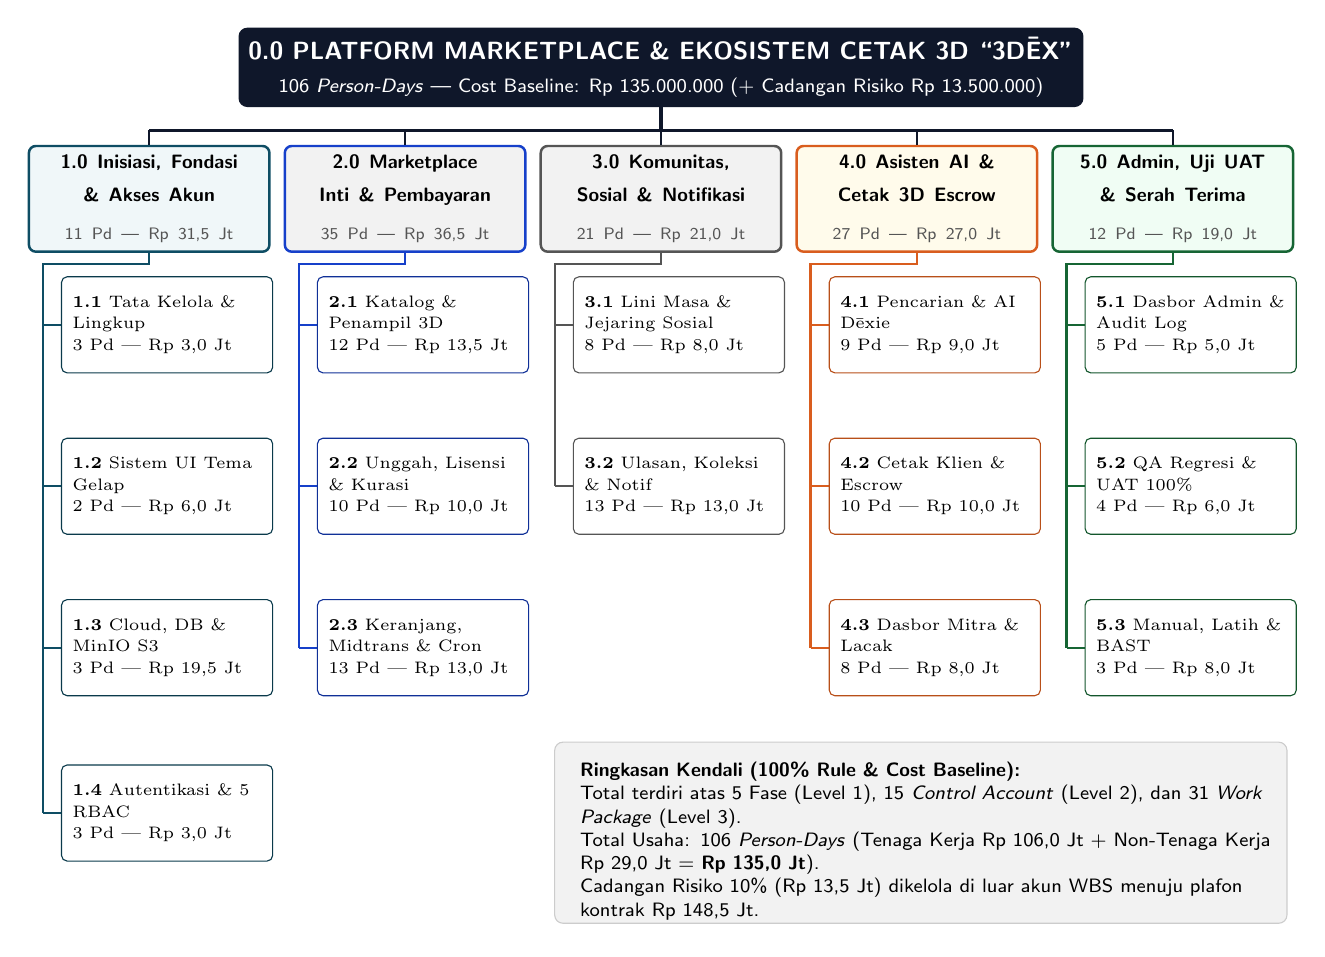
\begin{tikzpicture}[font=\sffamily]
    % Define column center coordinates for 5 major phases across 16.2cm width
    % Centers: 1.60, 4.85, 8.10, 11.35, 14.60 (col spacing 3.25cm, card width 2.85cm)
    \def\rooty{12.22}
    \def\loney{10.55}

    % Level 0 Root Node (width 10.2cm centered at x=8.10)
    \node[draw=brandnavy, fill=brandnavy, text=white, rounded corners=3pt,
          minimum width=10.2cm, minimum height=0.95cm, align=center] (root) at (8.10, \rooty)
          {{\small\bfseries 0.0 PLATFORM MARKETPLACE \& EKOSISTEM CETAK 3D ``3D\={E}X''}\\
           {\scriptsize 106 \textit{Person-Days} | Cost Baseline: Rp 135.000.000 (+ Cadangan Risiko Rp 13.500.000)}};

    % Trunk down from root to horizontal bus at y=11.42
    \draw[brandnavy, line width=1.1pt] (root.south) -- (8.10, 11.42);
    \draw[brandnavy, line width=1.1pt] (1.60, 11.42) -- (14.60, 11.42);

    % Level 1 Phase Nodes (5 columns) anchored explicitly via (l1_\idx) so connectors never penetrate boxes
    \foreach \idx/\cx/\code/\title/\meta/\col/\fillcol in {
        1/1.60/1.0/{Inisiasi, Fondasi \& Akses Akun}/{11 Pd | Rp 31,5 Jt}/accentteal/softteal,
        2/4.85/2.0/{Marketplace Inti \& Pembayaran}/{35 Pd | Rp 36,5 Jt}/brandblue/lightslate,
        3/8.10/3.0/{Komunitas, Sosial \& Notifikasi}/{21 Pd | Rp 21,0 Jt}/mutedtext/lightslate,
        4/11.35/4.0/{Asisten AI \& Cetak 3D Escrow}/{27 Pd | Rp 27,0 Jt}/accentorange/softamber,
        5/14.60/5.0/{Admin, Uji UAT \& Serah Terima}/{12 Pd | Rp 19,0 Jt}/accentgreen/softgreen%
    } {
        \node[draw=\col, fill=\fillcol, line width=0.9pt, rounded corners=2.5pt,
              text width=2.82cm, minimum height=1.08cm, align=center] (l1_\idx) at (\cx, \loney)
              {{\scriptsize\bfseries\color{black}\code\ \title}\\[1.5pt]
               {\fontsize{6.2}{7.2}\selectfont\color{mutedtext}\meta}};
        \draw[brandnavy, line width=0.9pt] (\cx, 11.42) -- (l1_\idx.north);
    }

    % Spine helper per column: always starts strictly from (l1_\idx.south) down to y=9.72 above CAs
    % Column 1 Control Accounts (4 CAs)
    \def\sx{0.25}
    \draw[accentteal, line width=0.8pt] (l1_1.south) -- (1.60, 9.72) -- (\sx, 9.72) -- (\sx, 2.75);
    \foreach \cy/\lbl in {
        8.95/{{\bfseries 1.1} Tata Kelola \& Lingkup\\3 Pd | Rp 3,0 Jt},
        6.90/{{\bfseries 1.2} Sistem UI Tema Gelap\\2 Pd | Rp 6,0 Jt},
        4.85/{{\bfseries 1.3} Cloud, DB \& MinIO S3\\3 Pd | Rp 19,5 Jt},
        2.75/{{\bfseries 1.4} Autentikasi \& 5 RBAC\\3 Pd | Rp 3,0 Jt}
    } {
        \draw[accentteal, line width=0.8pt] (\sx, \cy) -- (0.48, \cy);
        \node[draw=accentteal!75!black, fill=white, rounded corners=2pt, anchor=west,
              text width=2.40cm, minimum height=1.22cm, align=left, inner sep=4pt,
              font=\fontsize{6.4}{7.8}\selectfont] at (0.48, \cy) {\lbl};
    }

    % Column 2 Control Accounts (3 CAs)
    \def\sx{3.50}
    \draw[brandblue, line width=0.8pt] (l1_2.south) -- (4.85, 9.72) -- (\sx, 9.72) -- (\sx, 4.85);
    \foreach \cy/\lbl in {
        8.95/{{\bfseries 2.1} Katalog \& Penampil 3D\\12 Pd | Rp 13,5 Jt},
        6.90/{{\bfseries 2.2} Unggah, Lisensi \& Kurasi\\10 Pd | Rp 10,0 Jt},
        4.85/{{\bfseries 2.3} Keranjang, Midtrans \& Cron\\13 Pd | Rp 13,0 Jt}
    } {
        \draw[brandblue, line width=0.8pt] (\sx, \cy) -- (3.73, \cy);
        \node[draw=brandblue!75!black, fill=white, rounded corners=2pt, anchor=west,
              text width=2.40cm, minimum height=1.22cm, align=left, inner sep=4pt,
              font=\fontsize{6.4}{7.8}\selectfont] at (3.73, \cy) {\lbl};
    }

    % Column 3 Control Accounts (2 CAs)
    \def\sx{6.75}
    \draw[mutedtext, line width=0.8pt] (l1_3.south) -- (8.10, 9.72) -- (\sx, 9.72) -- (\sx, 6.90);
    \foreach \cy/\lbl in {
        8.95/{{\bfseries 3.1} Lini Masa \& Jejaring Sosial\\8 Pd | Rp 8,0 Jt},
        6.90/{{\bfseries 3.2} Ulasan, Koleksi \& Notif\\13 Pd | Rp 13,0 Jt}
    } {
        \draw[mutedtext, line width=0.8pt] (\sx, \cy) -- (6.98, \cy);
        \node[draw=mutedtext, fill=white, rounded corners=2pt, anchor=west,
              text width=2.40cm, minimum height=1.22cm, align=left, inner sep=4pt,
              font=\fontsize{6.4}{7.8}\selectfont] at (6.98, \cy) {\lbl};
    }

    % Column 4 Control Accounts (3 CAs)
    \def\sx{10.00}
    \draw[accentorange, line width=0.8pt] (l1_4.south) -- (11.35, 9.72) -- (\sx, 9.72) -- (\sx, 4.85);
    \foreach \cy/\lbl in {
        8.95/{{\bfseries 4.1} Pencarian \& AI D\={e}xie\\9 Pd | Rp 9,0 Jt},
        6.90/{{\bfseries 4.2} Cetak Klien \& Escrow\\10 Pd | Rp 10,0 Jt},
        4.85/{{\bfseries 4.3} Dasbor Mitra \& Lacak\\8 Pd | Rp 8,0 Jt}
    } {
        \draw[accentorange, line width=0.8pt] (\sx, \cy) -- (10.23, \cy);
        \node[draw=accentorange!85!black, fill=white, rounded corners=2pt, anchor=west,
              text width=2.40cm, minimum height=1.22cm, align=left, inner sep=4pt,
              font=\fontsize{6.4}{7.8}\selectfont] at (10.23, \cy) {\lbl};
    }

    % Column 5 Control Accounts (3 CAs)
    \def\sx{13.25}
    \draw[accentgreen, line width=0.8pt] (l1_5.south) -- (14.60, 9.72) -- (\sx, 9.72) -- (\sx, 4.85);
    \foreach \cy/\lbl in {
        8.95/{{\bfseries 5.1} Dasbor Admin \& Audit Log\\5 Pd | Rp 5,0 Jt},
        6.90/{{\bfseries 5.2} QA Regresi \& UAT 100\%\\4 Pd | Rp 6,0 Jt},
        4.85/{{\bfseries 5.3} Manual, Latih \& BAST\\3 Pd | Rp 8,0 Jt}
    } {
        \draw[accentgreen, line width=0.8pt] (\sx, \cy) -- (13.48, \cy);
        \node[draw=accentgreen!85!black, fill=white, rounded corners=2pt, anchor=west,
              text width=2.40cm, minimum height=1.22cm, align=left, inner sep=4pt,
              font=\fontsize{6.4}{7.8}\selectfont] at (13.48, \cy) {\lbl};
    }

    % Explanatory footer legend box spanning columns 3-5 empty bottom region cleanly
    \fill[lightslate, rounded corners=3pt] (6.75, 1.35) rectangle (16.05, 3.65);
    \draw[bordergray, rounded corners=3pt] (6.75, 1.35) rectangle (16.05, 3.65);
    \node[anchor=north west, text width=8.9cm, font=\sffamily\fontsize{6.6}{8.4}\selectfont, text=black, align=left] at (6.95, 3.52)
         {\textbf{Ringkasan Kendali (\textit{100\% Rule} \& \textit{Cost Baseline}):}\\
          Total terdiri atas 5 Fase (Level 1), 15 \textit{Control Account} (Level 2), dan 31 \textit{Work Package} (Level 3).\\
          Total Usaha: 106 \textit{Person-Days} (Tenaga Kerja Rp 106,0 Jt + Non-Tenaga Kerja Rp 29,0 Jt = \textbf{Rp 135,0 Jt}).\\
          Cadangan Risiko 10\% (Rp 13,5 Jt) dikelola di luar akun WBS menuju plafon kontrak Rp 148,5 Jt.};
\end{tikzpicture}
\caption{Diagram Struktur Hierarki WBS Eksekutif Tingkat 0 s.d. Tingkat 2 (\textit{Control Accounts})}
\label{fig:wbs_exec_tree}
\end{figure}

\clearpage

\begin{figure}[H]
\centering
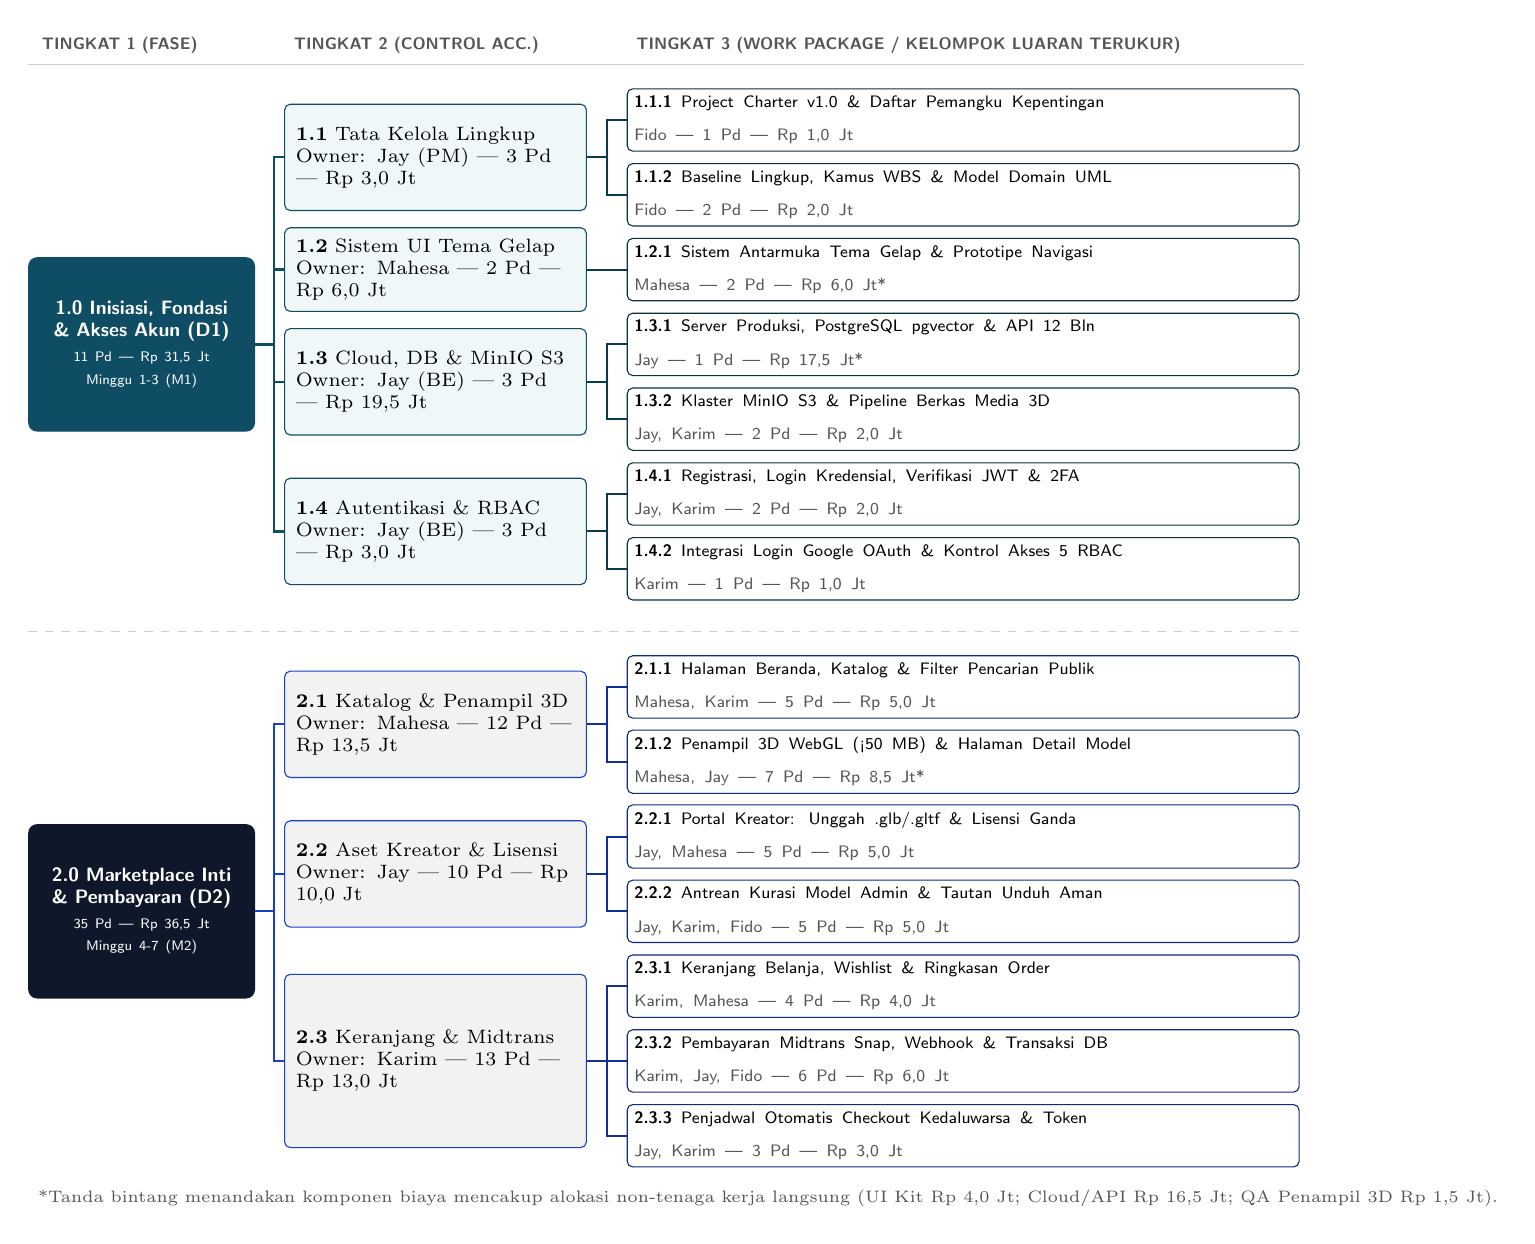
\begin{tikzpicture}[font=\sffamily]
    % Horizontal orthogonal hierarchy for Branch 1.0 (7 WPs) and Branch 2.0 (7 WPs) = 14 rows
    % Width strictly 16.2cm: L1 (0..2.75), L2 (3.25..7.05), L3 (7.60..16.20)

    % Column headers
    \node[anchor=west, font=\sffamily\fontsize{6.3}{7.3}\selectfont\bfseries, text=mutedtext] at (0.05, 16.2) {TINGKAT 1 (FASE)};
    \node[anchor=west, font=\sffamily\fontsize{6.3}{7.3}\selectfont\bfseries, text=mutedtext] at (3.25, 16.2) {TINGKAT 2 (CONTROL ACC.)};
    \node[anchor=west, font=\sffamily\fontsize{6.3}{7.3}\selectfont\bfseries, text=mutedtext] at (7.60, 16.2) {TINGKAT 3 (\textit{WORK PACKAGE} / KELOMPOK LUARAN TERUKUR)};
    \draw[bordergray] (0, 15.95) -- (16.2, 15.95);

    % ---- BRANCH 1.0 (Rows y=15.35 down to 9.35 -> 7 WPs) ----
    \foreach \idx/\y/\code/\title/\meta in {
        1/15.25/1.1.1/{Project Charter v1.0 \& Daftar Pemangku Kepentingan}/{Fido | 1 Pd | Rp 1,0 Jt},
        2/14.30/1.1.2/{Baseline Lingkup, Kamus WBS \& Model Domain UML}/{Fido | 2 Pd | Rp 2,0 Jt},
        3/13.35/1.2.1/{Sistem Antarmuka Tema Gelap \& Prototipe Navigasi}/{Mahesa | 2 Pd | Rp 6,0 Jt*},
        4/12.40/1.3.1/{Server Produksi, PostgreSQL pgvector \& API 12 Bln}/{Jay | 1 Pd | Rp 17,5 Jt*},
        5/11.45/1.3.2/{Klaster MinIO S3 \& Pipeline Berkas Media 3D}/{Jay, Karim | 2 Pd | Rp 2,0 Jt},
        6/10.50/1.4.1/{Registrasi, Login Kredensial, Verifikasi JWT \& 2FA}/{Jay, Karim | 2 Pd | Rp 2,0 Jt},
        7/9.55/1.4.2/{Integrasi Login Google OAuth \& Kontrol Akses 5 RBAC}/{Karim | 1 Pd | Rp 1,0 Jt}%
    } {
        \node[draw=accentteal!65!black, fill=white, rounded corners=2pt, anchor=west,
              text width=8.35cm, minimum height=0.72cm, align=left, inner sep=2.6pt] (wp1\idx) at (7.60, \y)
              {{\fontsize{6.5}{7.5}\selectfont\textbf{\code}\ \title}\\{\fontsize{6.0}{7.0}\selectfont\color{mutedtext}\meta}};
    }

    % Branch 1.0 Level 2 Control Accounts
    \node[draw=accentteal, fill=softteal, rounded corners=2pt, anchor=west, text width=3.55cm, minimum height=1.35cm, align=left, inner sep=4pt, font=\fontsize{6.7}{8.0}\selectfont] (ca11) at (3.25, 14.775)
         {\textbf{1.1} Tata Kelola Lingkup\\Owner: Jay (PM) | 3 Pd | Rp 3,0 Jt};
    \node[draw=accentteal, fill=softteal, rounded corners=2pt, anchor=west, text width=3.55cm, minimum height=0.74cm, align=left, inner sep=4pt, font=\fontsize{6.7}{8.0}\selectfont] (ca12) at (3.25, 13.35)
         {\textbf{1.2} Sistem UI Tema Gelap\\Owner: Mahesa | 2 Pd | Rp 6,0 Jt};
    \node[draw=accentteal, fill=softteal, rounded corners=2pt, anchor=west, text width=3.55cm, minimum height=1.35cm, align=left, inner sep=4pt, font=\fontsize{6.7}{8.0}\selectfont] (ca13) at (3.25, 11.925)
         {\textbf{1.3} Cloud, DB \& MinIO S3\\Owner: Jay (BE) | 3 Pd | Rp 19,5 Jt};
    \node[draw=accentteal, fill=softteal, rounded corners=2pt, anchor=west, text width=3.55cm, minimum height=1.35cm, align=left, inner sep=4pt, font=\fontsize{6.7}{8.0}\selectfont] (ca14) at (3.25, 10.025)
         {\textbf{1.4} Autentikasi \& RBAC\\Owner: Jay (BE) | 3 Pd | Rp 3,0 Jt};

    % Branch 1.0 Level 1 Node
    \node[draw=accentteal, fill=accentteal, text=white, rounded corners=3pt, anchor=west, text width=2.62cm, minimum height=2.2cm, align=center, inner sep=3.5pt, font=\sffamily\scriptsize] (b1) at (0, 12.40)
         {\textbf{1.0 Inisiasi, Fondasi \& Akses Akun (D1)}\\[3pt]{\tiny 11 Pd | Rp 31,5 Jt\\Minggu 1-3 (M1)}};

    % Connectors Branch 1.0
    \foreach \ca in {ca11, ca12, ca13, ca14} {
        \draw[accentteal, line width=0.8pt] (b1.east) -- ++(0.24,0) |- (\ca.west);
    }
    \draw[accentteal!75!black, line width=0.7pt] (ca11.east) -- ++(0.25,0) |- (wp11.west);
    \draw[accentteal!75!black, line width=0.7pt] (ca11.east) -- ++(0.25,0) |- (wp12.west);
    \draw[accentteal!75!black, line width=0.7pt] (ca12.east) -- (wp13.west);
    \draw[accentteal!75!black, line width=0.7pt] (ca13.east) -- ++(0.25,0) |- (wp14.west);
    \draw[accentteal!75!black, line width=0.7pt] (ca13.east) -- ++(0.25,0) |- (wp15.west);
    \draw[accentteal!75!black, line width=0.7pt] (ca14.east) -- ++(0.25,0) |- (wp16.west);
    \draw[accentteal!75!black, line width=0.7pt] (ca14.east) -- ++(0.25,0) |- (wp17.west);

    % Subtle separator between Branch 1.0 and 2.0
    \draw[bordergray, dashed] (0, 8.75) -- (16.2, 8.75);

    % ---- BRANCH 2.0 (Rows y=8.15 down to 2.25 -> 7 WPs) ----
    \foreach \idx/\y/\code/\title/\meta in {
        1/8.05/2.1.1/{Halaman Beranda, Katalog \& Filter Pencarian Publik}/{Mahesa, Karim | 5 Pd | Rp 5,0 Jt},
        2/7.10/2.1.2/{Penampil 3D WebGL (<50 MB) \& Halaman Detail Model}/{Mahesa, Jay | 7 Pd | Rp 8,5 Jt*},
        3/6.15/2.2.1/{Portal Kreator: Unggah .glb/.gltf \& Lisensi Ganda}/{Jay, Mahesa | 5 Pd | Rp 5,0 Jt},
        4/5.20/2.2.2/{Antrean Kurasi Model Admin \& Tautan Unduh Aman}/{Jay, Karim, Fido | 5 Pd | Rp 5,0 Jt},
        5/4.25/2.3.1/{Keranjang Belanja, Wishlist \& Ringkasan Order}/{Karim, Mahesa | 4 Pd | Rp 4,0 Jt},
        6/3.30/2.3.2/{Pembayaran Midtrans Snap, Webhook \& Transaksi DB}/{Karim, Jay, Fido | 6 Pd | Rp 6,0 Jt},
        7/2.35/2.3.3/{Penjadwal Otomatis Checkout Kedaluwarsa \& Token}/{Jay, Karim | 3 Pd | Rp 3,0 Jt}%
    } {
        \node[draw=brandblue!65!black, fill=white, rounded corners=2pt, anchor=west,
              text width=8.35cm, minimum height=0.72cm, align=left, inner sep=2.6pt] (wp2\idx) at (7.60, \y)
              {{\fontsize{6.5}{7.5}\selectfont\textbf{\code}\ \title}\\{\fontsize{6.0}{7.0}\selectfont\color{mutedtext}\meta}};
    }

    \node[draw=brandblue, fill=lightslate, rounded corners=2pt, anchor=west, text width=3.55cm, minimum height=1.35cm, align=left, inner sep=4pt, font=\fontsize{6.7}{8.0}\selectfont] (ca21) at (3.25, 7.575)
         {\textbf{2.1} Katalog \& Penampil 3D\\Owner: Mahesa | 12 Pd | Rp 13,5 Jt};
    \node[draw=brandblue, fill=lightslate, rounded corners=2pt, anchor=west, text width=3.55cm, minimum height=1.35cm, align=left, inner sep=4pt, font=\fontsize{6.7}{8.0}\selectfont] (ca22) at (3.25, 5.675)
         {\textbf{2.2} Aset Kreator \& Lisensi\\Owner: Jay | 10 Pd | Rp 10,0 Jt};
    \node[draw=brandblue, fill=lightslate, rounded corners=2pt, anchor=west, text width=3.55cm, minimum height=2.20cm, align=left, inner sep=4pt, font=\fontsize{6.7}{8.0}\selectfont] (ca23) at (3.25, 3.30)
         {\textbf{2.3} Keranjang \& Midtrans\\Owner: Karim | 13 Pd | Rp 13,0 Jt};

    \node[draw=brandnavy, fill=brandnavy, text=white, rounded corners=3pt, anchor=west, text width=2.62cm, minimum height=2.2cm, align=center, inner sep=3.5pt, font=\sffamily\scriptsize] (b2) at (0, 5.20)
         {\textbf{2.0 Marketplace Inti \& Pembayaran (D2)}\\[3pt]{\tiny 35 Pd | Rp 36,5 Jt\\Minggu 4-7 (M2)}};

    \foreach \ca in {ca21, ca22, ca23} {
        \draw[brandblue, line width=0.8pt] (b2.east) -- ++(0.24,0) |- (\ca.west);
    }
    \draw[brandblue!75!black, line width=0.7pt] (ca21.east) -- ++(0.25,0) |- (wp21.west);
    \draw[brandblue!75!black, line width=0.7pt] (ca21.east) -- ++(0.25,0) |- (wp22.west);
    \draw[brandblue!75!black, line width=0.7pt] (ca22.east) -- ++(0.25,0) |- (wp23.west);
    \draw[brandblue!75!black, line width=0.7pt] (ca22.east) -- ++(0.25,0) |- (wp24.west);
    \draw[brandblue!75!black, line width=0.7pt] (ca23.east) -- ++(0.25,0) |- (wp25.west);
    \draw[brandblue!75!black, line width=0.7pt] (ca23.east) -- ++(0.25,0) |- (wp26.west);
    \draw[brandblue!75!black, line width=0.7pt] (ca23.east) -- ++(0.25,0) |- (wp27.west);

    % Note at bottom
    \node[anchor=west, font=\fontsize{6.5}{7.5}\selectfont\color{mutedtext}] at (0, 1.55)
         {*Tanda bintang menandakan komponen biaya mencakup alokasi non-tenaga kerja langsung (UI Kit Rp 4,0 Jt; Cloud/API Rp 16,5 Jt; QA Penampil 3D Rp 1,5 Jt).};
\end{tikzpicture}
\caption{Dekomposisi Detail \textit{Work Package} Cabang 1.0 dan Cabang 2.0 (14 \textit{Work Package})}
\label{fig:wbs_detail_12}
\end{figure}

\clearpage

\begin{figure}[H]
\centering
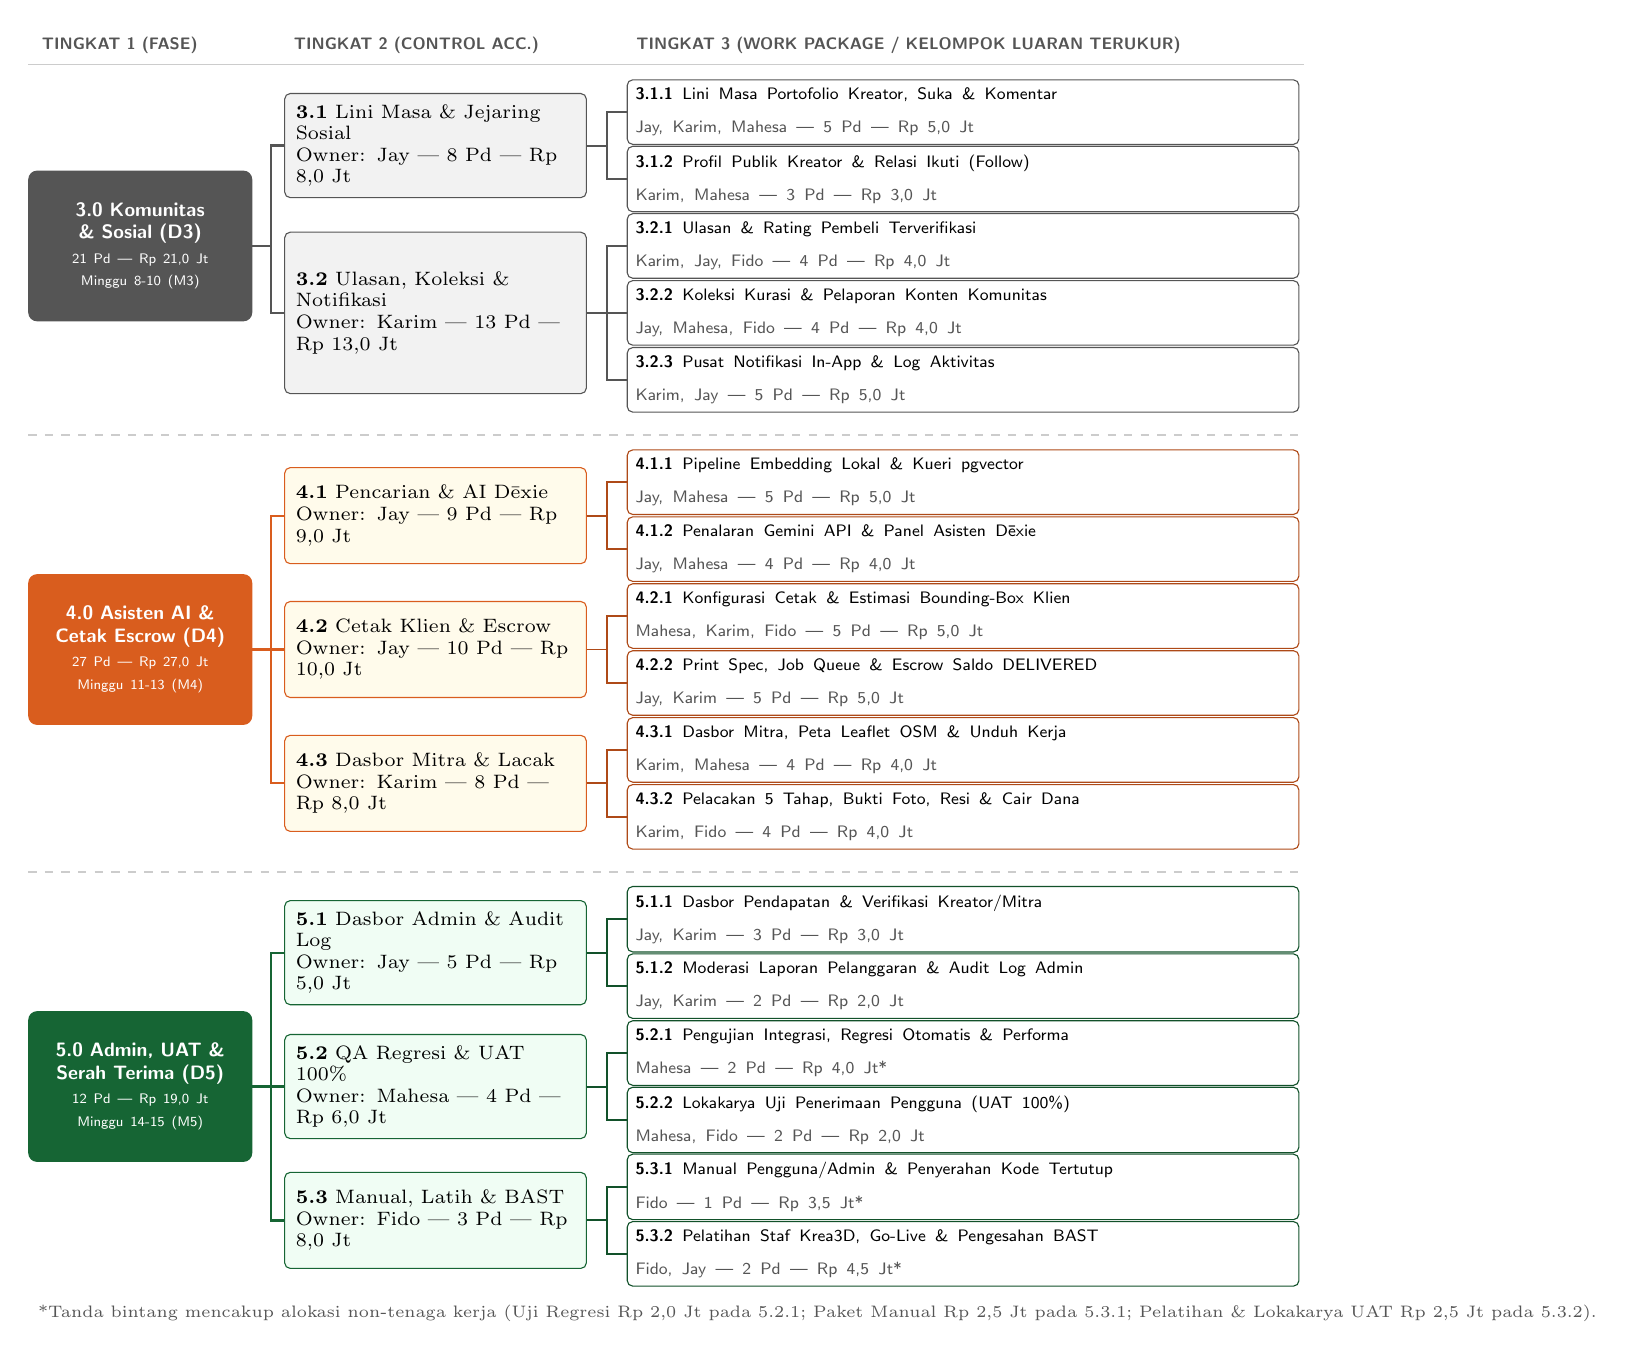
\begin{tikzpicture}[font=\sffamily]
    % Horizontal orthogonal hierarchy for Branches 3.0 (5 WPs), 4.0 (6 WPs), 5.0 (6 WPs) = 17 rows
    \node[anchor=west, font=\sffamily\fontsize{6.3}{7.3}\selectfont\bfseries, text=mutedtext] at (0.05, 17.55) {TINGKAT 1 (FASE)};
    \node[anchor=west, font=\sffamily\fontsize{6.3}{7.3}\selectfont\bfseries, text=mutedtext] at (3.25, 17.55) {TINGKAT 2 (CONTROL ACC.)};
    \node[anchor=west, font=\sffamily\fontsize{6.3}{7.3}\selectfont\bfseries, text=mutedtext] at (7.60, 17.55) {TINGKAT 3 (\textit{WORK PACKAGE} / KELOMPOK LUARAN TERUKUR)};
    \draw[bordergray] (0, 17.30) -- (16.2, 17.30);

    % ---- BRANCH 3.0 (5 WPs: y=16.70 down to 13.30, pitch 0.85) ----
    \foreach \idx/\y/\code/\title/\meta in {
        1/16.70/3.1.1/{Lini Masa Portofolio Kreator, Suka \& Komentar}/{Jay, Karim, Mahesa | 5 Pd | Rp 5,0 Jt},
        2/15.85/3.1.2/{Profil Publik Kreator \& Relasi Ikuti (Follow)}/{Karim, Mahesa | 3 Pd | Rp 3,0 Jt},
        3/15.00/3.2.1/{Ulasan \& Rating Pembeli Terverifikasi}/{Karim, Jay, Fido | 4 Pd | Rp 4,0 Jt},
        4/14.15/3.2.2/{Koleksi Kurasi \& Pelaporan Konten Komunitas}/{Jay, Mahesa, Fido | 4 Pd | Rp 4,0 Jt},
        5/13.30/3.2.3/{Pusat Notifikasi In-App \& Log Aktivitas}/{Karim, Jay | 5 Pd | Rp 5,0 Jt}%
    } {
        \node[draw=mutedtext, fill=white, rounded corners=2pt, anchor=west,
              text width=8.32cm, minimum height=0.66cm, align=left, inner sep=3pt] (wp3\idx) at (7.60, \y)
              {{\fontsize{6.4}{7.2}\selectfont\textbf{\code}\ \title}\\{\fontsize{5.8}{6.6}\selectfont\color{mutedtext}\meta}};
    }
    \node[draw=mutedtext, fill=lightslate, rounded corners=2pt, anchor=west, text width=3.55cm, minimum height=1.22cm, align=left, inner sep=4pt, font=\fontsize{6.6}{7.8}\selectfont] (ca31) at (3.25, 16.275)
         {\textbf{3.1} Lini Masa \& Jejaring Sosial\\Owner: Jay | 8 Pd | Rp 8,0 Jt};
    \node[draw=mutedtext, fill=lightslate, rounded corners=2pt, anchor=west, text width=3.55cm, minimum height=2.05cm, align=left, inner sep=4pt, font=\fontsize{6.6}{7.8}\selectfont] (ca32) at (3.25, 14.15)
         {\textbf{3.2} Ulasan, Koleksi \& Notifikasi\\Owner: Karim | 13 Pd | Rp 13,0 Jt};
    \node[draw=mutedtext, fill=mutedtext, text=white, rounded corners=3pt, anchor=west, text width=2.55cm, minimum height=1.9cm, align=center, inner sep=4pt, font=\sffamily\scriptsize] (b3) at (0, 15.00)
         {\textbf{3.0 Komunitas \& Sosial (D3)}\\[3pt]{\tiny 21 Pd | Rp 21,0 Jt\\Minggu 8-10 (M3)}};

    \foreach \ca in {ca31, ca32} { \draw[mutedtext, line width=0.8pt] (b3.east) -- ++(0.24,0) |- (\ca.west); }
    \draw[mutedtext, line width=0.7pt] (ca31.east) -- ++(0.25,0) |- (wp31.west);
    \draw[mutedtext, line width=0.7pt] (ca31.east) -- ++(0.25,0) |- (wp32.west);
    \draw[mutedtext, line width=0.7pt] (ca32.east) -- ++(0.25,0) |- (wp33.west);
    \draw[mutedtext, line width=0.7pt] (ca32.east) -- (wp34.west);
    \draw[mutedtext, line width=0.7pt] (ca32.east) -- ++(0.25,0) |- (wp35.west);

    \draw[bordergray, dashed] (0, 12.60) -- (16.2, 12.60);

    % ---- BRANCH 4.0 (6 WPs: y=12.00 down to 7.75, pitch 0.85) ----
    \foreach \idx/\y/\code/\title/\meta in {
        1/12.00/4.1.1/{Pipeline Embedding Lokal \& Kueri pgvector}/{Jay, Mahesa | 5 Pd | Rp 5,0 Jt},
        2/11.15/4.1.2/{Penalaran Gemini API \& Panel Asisten D\={e}xie}/{Jay, Mahesa | 4 Pd | Rp 4,0 Jt},
        3/10.30/4.2.1/{Konfigurasi Cetak \& Estimasi Bounding-Box Klien}/{Mahesa, Karim, Fido | 5 Pd | Rp 5,0 Jt},
        4/9.45/4.2.2/{Print Spec, Job Queue \& Escrow Saldo DELIVERED}/{Jay, Karim | 5 Pd | Rp 5,0 Jt},
        5/8.60/4.3.1/{Dasbor Mitra, Peta Leaflet OSM \& Unduh Kerja}/{Karim, Mahesa | 4 Pd | Rp 4,0 Jt},
        6/7.75/4.3.2/{Pelacakan 5 Tahap, Bukti Foto, Resi \& Cair Dana}/{Karim, Fido | 4 Pd | Rp 4,0 Jt}%
    } {
        \node[draw=accentorange!80!black, fill=white, rounded corners=2pt, anchor=west,
              text width=8.32cm, minimum height=0.66cm, align=left, inner sep=3pt] (wp4\idx) at (7.60, \y)
              {{\fontsize{6.4}{7.2}\selectfont\textbf{\code}\ \title}\\{\fontsize{5.8}{6.6}\selectfont\color{mutedtext}\meta}};
    }
    \node[draw=accentorange, fill=softamber, rounded corners=2pt, anchor=west, text width=3.55cm, minimum height=1.22cm, align=left, inner sep=4pt, font=\fontsize{6.6}{7.8}\selectfont] (ca41) at (3.25, 11.575)
         {\textbf{4.1} Pencarian \& AI D\={e}xie\\Owner: Jay | 9 Pd | Rp 9,0 Jt};
    \node[draw=accentorange, fill=softamber, rounded corners=2pt, anchor=west, text width=3.55cm, minimum height=1.22cm, align=left, inner sep=4pt, font=\fontsize{6.6}{7.8}\selectfont] (ca42) at (3.25, 9.875)
         {\textbf{4.2} Cetak Klien \& Escrow\\Owner: Jay | 10 Pd | Rp 10,0 Jt};
    \node[draw=accentorange, fill=softamber, rounded corners=2pt, anchor=west, text width=3.55cm, minimum height=1.22cm, align=left, inner sep=4pt, font=\fontsize{6.6}{7.8}\selectfont] (ca43) at (3.25, 8.175)
         {\textbf{4.3} Dasbor Mitra \& Lacak\\Owner: Karim | 8 Pd | Rp 8,0 Jt};
    \node[draw=accentorange, fill=accentorange, text=white, rounded corners=3pt, anchor=west, text width=2.55cm, minimum height=1.9cm, align=center, inner sep=4pt, font=\sffamily\scriptsize] (b4) at (0, 9.875)
         {\textbf{4.0 Asisten AI \& Cetak Escrow (D4)}\\[3pt]{\tiny 27 Pd | Rp 27,0 Jt\\Minggu 11-13 (M4)}};

    \foreach \ca in {ca41, ca42, ca43} { \draw[accentorange, line width=0.8pt] (b4.east) -- ++(0.24,0) |- (\ca.west); }
    \draw[accentorange!80!black, line width=0.7pt] (ca41.east) -- ++(0.25,0) |- (wp41.west);
    \draw[accentorange!80!black, line width=0.7pt] (ca41.east) -- ++(0.25,0) |- (wp42.west);
    \draw[accentorange!80!black, line width=0.7pt] (ca42.east) -- ++(0.25,0) |- (wp43.west);
    \draw[accentorange!80!black, line width=0.7pt] (ca42.east) -- ++(0.25,0) |- (wp44.west);
    \draw[accentorange!80!black, line width=0.7pt] (ca43.east) -- ++(0.25,0) |- (wp45.west);
    \draw[accentorange!80!black, line width=0.7pt] (ca43.east) -- ++(0.25,0) |- (wp46.west);

    \draw[bordergray, dashed] (0, 7.05) -- (16.2, 7.05);

    % ---- BRANCH 5.0 (6 WPs: y=6.45 down to 2.20, pitch 0.85) ----
    \foreach \idx/\y/\code/\title/\meta in {
        1/6.45/5.1.1/{Dasbor Pendapatan \& Verifikasi Kreator/Mitra}/{Jay, Karim | 3 Pd | Rp 3,0 Jt},
        2/5.60/5.1.2/{Moderasi Laporan Pelanggaran \& Audit Log Admin}/{Jay, Karim | 2 Pd | Rp 2,0 Jt},
        3/4.75/5.2.1/{Pengujian Integrasi, Regresi Otomatis \& Performa}/{Mahesa | 2 Pd | Rp 4,0 Jt*},
        4/3.90/5.2.2/{Lokakarya Uji Penerimaan Pengguna (UAT 100\%)}/{Mahesa, Fido | 2 Pd | Rp 2,0 Jt},
        5/3.05/5.3.1/{Manual Pengguna/Admin \& Penyerahan Kode Tertutup}/{Fido | 1 Pd | Rp 3,5 Jt*},
        6/2.20/5.3.2/{Pelatihan Staf Krea3D, Go-Live \& Pengesahan BAST}/{Fido, Jay | 2 Pd | Rp 4,5 Jt*}%
    } {
        \node[draw=accentgreen!80!black, fill=white, rounded corners=2pt, anchor=west,
              text width=8.32cm, minimum height=0.66cm, align=left, inner sep=3pt] (wp5\idx) at (7.60, \y)
              {{\fontsize{6.4}{7.2}\selectfont\textbf{\code}\ \title}\\{\fontsize{5.8}{6.6}\selectfont\color{mutedtext}\meta}};
    }
    \node[draw=accentgreen, fill=softgreen, rounded corners=2pt, anchor=west, text width=3.55cm, minimum height=1.22cm, align=left, inner sep=4pt, font=\fontsize{6.6}{7.8}\selectfont] (ca51) at (3.25, 6.025)
         {\textbf{5.1} Dasbor Admin \& Audit Log\\Owner: Jay | 5 Pd | Rp 5,0 Jt};
    \node[draw=accentgreen, fill=softgreen, rounded corners=2pt, anchor=west, text width=3.55cm, minimum height=1.22cm, align=left, inner sep=4pt, font=\fontsize{6.6}{7.8}\selectfont] (ca52) at (3.25, 4.325)
         {\textbf{5.2} QA Regresi \& UAT 100\%\\Owner: Mahesa | 4 Pd | Rp 6,0 Jt};
    \node[draw=accentgreen, fill=softgreen, rounded corners=2pt, anchor=west, text width=3.55cm, minimum height=1.22cm, align=left, inner sep=4pt, font=\fontsize{6.6}{7.8}\selectfont] (ca53) at (3.25, 2.625)
         {\textbf{5.3} Manual, Latih \& BAST\\Owner: Fido | 3 Pd | Rp 8,0 Jt};
    \node[draw=accentgreen, fill=accentgreen, text=white, rounded corners=3pt, anchor=west, text width=2.55cm, minimum height=1.9cm, align=center, inner sep=4pt, font=\sffamily\scriptsize] (b5) at (0, 4.325)
         {\textbf{5.0 Admin, UAT \& Serah Terima (D5)}\\[3pt]{\tiny 12 Pd | Rp 19,0 Jt\\Minggu 14-15 (M5)}};

    \foreach \ca in {ca51, ca52, ca53} { \draw[accentgreen, line width=0.8pt] (b5.east) -- ++(0.24,0) |- (\ca.west); }
    \draw[accentgreen!80!black, line width=0.7pt] (ca51.east) -- ++(0.25,0) |- (wp51.west);
    \draw[accentgreen!80!black, line width=0.7pt] (ca51.east) -- ++(0.25,0) |- (wp52.west);
    \draw[accentgreen!80!black, line width=0.7pt] (ca52.east) -- ++(0.25,0) |- (wp53.west);
    \draw[accentgreen!80!black, line width=0.7pt] (ca52.east) -- ++(0.25,0) |- (wp54.west);
    \draw[accentgreen!80!black, line width=0.7pt] (ca53.east) -- ++(0.25,0) |- (wp55.west);
    \draw[accentgreen!80!black, line width=0.7pt] (ca53.east) -- ++(0.25,0) |- (wp56.west);

    \node[anchor=west, font=\fontsize{6.5}{7.5}\selectfont\color{mutedtext}] at (0, 1.45)
         {*Tanda bintang mencakup alokasi non-tenaga kerja (Uji Regresi Rp 2,0 Jt pada 5.2.1; Paket Manual Rp 2,5 Jt pada 5.3.1; Pelatihan \& Lokakarya UAT Rp 2,5 Jt pada 5.3.2).};
\end{tikzpicture}
\caption{Dekomposisi Detail \textit{Work Package} Cabang 3.0, 4.0, dan 5.0 (17 \textit{Work Package})}
\label{fig:wbs_detail_345}
\end{figure}

\clearpage

% ==============================================================================
% BAB 3: WBS TERSTRUKTUR (TABULAR OUTLINE) & MATRIKS GULUNG BIAYA / USAHA
% ==============================================================================
\section{WBS Terstruktur (\textit{Tabular Outline}) dan Matriks Gulung Biaya}

Tabel \ref{tab:wbs_rollup} menyajikan keseluruhan struktur WBS secara berjenjang dari tingkat atas hingga seluruh 31 \textit{Work Package} (\textit{bottom-up roll-up}), membuktikan kepatuhan penuh terhadap Aturan 100\% serta kesesuaian mutlak terhadap anggaran dasar Rp 135.000.000.

{\renewcommand{\arraystretch}{1.12}\setlength{\tabcolsep}{3.0pt}\setlength{\LTcapwidth}{\textwidth}\scriptsize
\begin{longtable}{| C{0.85cm} | C{0.90cm} | L{4.80cm} | L{1.90cm} | C{0.90cm} | R{1.65cm} | R{1.65cm} | R{1.90cm} |}
\caption{WBS Terstruktur Lengkap dan Matriks Gulung Usaha (\textit{Pd}) serta Biaya Baseline (IDR)} \label{tab:wbs_rollup} \\
\hline
\rowcolor{tableheadergray} \thdr{Kode} & \thdr{Tipe} & \thdr{Nama Komponen Deliverable WBS} & \thdr{Pemilik (CAM)} & \thdr{Usaha (Pd)} & \thdr{Biaya Tenaga Kerja} & \thdr{Non-Tenaga Kerja} & \thdr{Total Baseline (Rp)} \\
\hline
\endfirsthead
\hline
\rowcolor{tableheadergray} \thdr{Kode} & \thdr{Tipe} & \thdr{Nama Komponen Deliverable WBS} & \thdr{Pemilik (CAM)} & \thdr{Usaha (Pd)} & \thdr{Biaya Tenaga Kerja} & \thdr{Non-Tenaga Kerja} & \thdr{Total Baseline (Rp)} \\
\hline
\endhead
\hline
\multicolumn{8}{|r|}{\textit{Bersambung ke halaman berikutnya...}} \\
\hline
\endfoot
\hline
\endlastfoot

% BRANCH 1.0
\rowcolor{lightslate} \textbf{1.0} & L1-F1 & \textbf{Tata Kelola, Fondasi Infrastruktur \& Akses Akun (D1)} & Jay (PM) & 11 & 11.000.000 & 20.500.000 & \textbf{31.500.000} \\
\hline
1.1 & L2-CA & Tata Kelola Lingkup \& Spesifikasi Awal & Jay (PM) & 3 & 3.000.000 & 0 & 3.000.000 \\
\hline
1.1.1 & L3-WP & Dokumen Project Charter v1.0 \& Daftar Pemangku Kepentingan & Fido (BA) & 1 & 1.000.000 & 0 & 1.000.000 \\
\hline
1.1.2 & L3-WP & Baseline Lingkup, Kamus WBS \& Model Domain UML & Fido (BA) & 2 & 2.000.000 & 0 & 2.000.000 \\
\hline
1.2 & L2-CA & Sistem Desain Antarmuka Tema Gelap \& UI Kit & Mahesa (FE) & 2 & 2.000.000 & 4.000.000 & 6.000.000 \\
\hline
1.2.1 & L3-WP & Prototipe Interaktif Antarmuka Gelap \& Navigasi Responsif & Mahesa (FE) & 2 & 2.000.000 & 4.000.000 & 6.000.000 \\
\hline
1.3 & L2-CA & Fondasi Infrastruktur Cloud, DB \& Penyimpanan S3 & Jay (BE) & 3 & 3.000.000 & 16.500.000 & 19.500.000 \\
\hline
1.3.1 & L3-WP & Server Produksi, PostgreSQL pgvector, SSL \& Kuota API 12 Bln & Jay (BE) & 1 & 1.000.000 & 16.500.000 & 17.500.000 \\
\hline
1.3.2 & L3-WP & Klaster MinIO S3 \& Pipeline Berkas Media/3D & Jay, Karim & 2 & 2.000.000 & 0 & 2.000.000 \\
\hline
1.4 & L2-CA & Sistem Identitas, Autentikasi \& Manajemen Peran & Jay (BE) & 3 & 3.000.000 & 0 & 3.000.000 \\
\hline
1.4.1 & L3-WP & Registrasi, Login Kredensial, Verifikasi JWT \& Keamanan 2FA & Jay, Karim & 2 & 2.000.000 & 0 & 2.000.000 \\
\hline
1.4.2 & L3-WP & Integrasi Login Google OAuth \& Kontrol Akses 5 Peran RBAC & Karim (Int.) & 1 & 1.000.000 & 0 & 1.000.000 \\
\hline

% BRANCH 2.0
\rowcolor{lightslate} \textbf{2.0} & L1-F2 & \textbf{Platform Marketplace Inti \& Pembayaran Midtrans (D2)} & Jay (PM) & 35 & 35.000.000 & 1.500.000 & \textbf{36.500.000} \\
\hline
2.1 & L2-CA & Katalog Publik \& Penampil Geometri 3D Interaktif & Mahesa (FE) & 12 & 12.000.000 & 1.500.000 & 13.500.000 \\
\hline
2.1.1 & L3-WP & Halaman Beranda, Katalog Kategori \& Filter Pencarian Publik & Mahesa, Karim & 5 & 5.000.000 & 0 & 5.000.000 \\
\hline
2.1.2 & L3-WP & Penampil 3D WebGL (< 50 MB) \& Halaman Detail Aset & Mahesa, Jay & 7 & 7.000.000 & 1.500.000 & 8.500.000 \\
\hline
2.2 & L2-CA & Sistem Unggah Kreator, Lisensi \& Persetujuan Aset & Jay (BE) & 10 & 10.000.000 & 0 & 10.000.000 \\
\hline
2.2.1 & L3-WP & Portal Kreator: Unggah .glb/.gltf \& Skema Lisensi Ganda & Jay, Mahesa & 5 & 5.000.000 & 0 & 5.000.000 \\
\hline
2.2.2 & L3-WP & Antrean Kurasi Model Admin \& Tautan Unduh Berbatas Waktu & Jay, Karim, Fido & 5 & 5.000.000 & 0 & 5.000.000 \\
\hline
2.3 & L2-CA & Keranjang Belanja, Wishlist \& Gerbang Pembayaran & Karim (Int.) & 13 & 13.000.000 & 0 & 13.000.000 \\
\hline
2.3.1 & L3-WP & Modul Keranjang Belanja, Wishlist \& Ringkasan Pesanan & Karim, Mahesa & 4 & 4.000.000 & 0 & 4.000.000 \\
\hline
2.3.2 & L3-WP & Midtrans Snap, Webhook Idempoten \& Transaksi DB Atomik & Karim, Jay, Fido & 6 & 6.000.000 & 0 & 6.000.000 \\
\hline
2.3.3 & L3-WP & Penjadwal Otomatis Pembatalan Checkout \& Token Sesi & Jay, Karim & 3 & 3.000.000 & 0 & 3.000.000 \\
\hline

% BRANCH 3.0
\rowcolor{lightslate} \textbf{3.0} & L1-F3 & \textbf{Ekosistem Komunitas, Interaksi Sosial \& Notifikasi (D3)} & Karim & 21 & 21.000.000 & 0 & \textbf{21.000.000} \\
\hline
3.1 & L2-CA & Lini Masa Komunitas \& Jejaring Sosial Kreator & Jay (BE) & 8 & 8.000.000 & 0 & 8.000.000 \\
\hline
3.1.1 & L3-WP & Lini Masa Publikasi Portofolio, Suka \& Thread Komentar & Jay, Karim, Mah. & 5 & 5.000.000 & 0 & 5.000.000 \\
\hline
3.1.2 & L3-WP & Profil Publik Kreator \& Mekanisme Ikuti (\textit{Follow/Unfollow}) & Karim, Mahesa & 3 & 3.000.000 & 0 & 3.000.000 \\
\hline
3.2 & L2-CA & Ulasan Terverifikasi, Koleksi \& Pusat Notifikasi & Karim (Int.) & 13 & 13.000.000 & 0 & 13.000.000 \\
\hline
3.2.1 & L3-WP & Ulasan \& Penilaian Aset Pembeli Resmi (\textit{Verified}) & Karim, Jay, Fido & 4 & 4.000.000 & 0 & 4.000.000 \\
\hline
3.2.2 & L3-WP & Koleksi Kurasi Pribadi/Publik \& Pelaporan Konten & Jay, Mah., Fido & 4 & 4.000.000 & 0 & 4.000.000 \\
\hline
3.2.3 & L3-WP & Pusat Notifikasi In-App \& Log Aktivitas Transaksional & Karim, Jay & 5 & 5.000.000 & 0 & 5.000.000 \\
\hline

% BRANCH 4.0
\rowcolor{lightslate} \textbf{4.0} & L1-F4 & \textbf{Asisten Cerdas AI D\={e}xie \& Layanan Cetak 3D Escrow (D4)} & Jay (PM) & 27 & 27.000.000 & 0 & \textbf{27.000.000} \\
\hline
4.1 & L2-CA & Mesin Pencarian Semantik \& Asisten AI D\={e}xie & Jay (BE) & 9 & 9.000.000 & 0 & 9.000.000 \\
\hline
4.1.1 & L3-WP & Pipeline Embedding Vektor Lokal \& Kueri Kosinus pgvector & Jay, Mahesa & 5 & 5.000.000 & 0 & 5.000.000 \\
\hline
4.1.2 & L3-WP & Penalaran Kontekstual Gemini API \& Panel Asisten D\={e}xie & Jay, Mahesa & 4 & 4.000.000 & 0 & 4.000.000 \\
\hline
4.2 & L2-CA & Konfigurasi Cetak Sisi Klien \& Penahanan Saldo Escrow & Jay (BE) & 10 & 10.000.000 & 0 & 10.000.000 \\
\hline
4.2.1 & L3-WP & Form Cetak 3D \& Kalkulator \textit{Bounding-Box} Klien & Mah., Kar., Fido & 5 & 5.000.000 & 0 & 5.000.000 \\
\hline
4.2.2 & L3-WP & Print Spec, Job Queue \& Buku Besar Escrow DELIVERED & Jay, Karim & 5 & 5.000.000 & 0 & 5.000.000 \\
\hline
4.3 & L2-CA & Dasbor Mitra Cetak, Lokasi \& Pelacakan 5 Tahap & Karim (Int.) & 8 & 8.000.000 & 0 & 8.000.000 \\
\hline
4.3.1 & L3-WP & Dasbor Antrean Mitra, Peta Leaflet/OSM \& Unduh Kerja & Karim, Mahesa & 4 & 4.000.000 & 0 & 4.000.000 \\
\hline
4.3.2 & L3-WP & Status 5 Tahap, Bukti Foto Cetak, Resi \& Pelepasan Dana & Karim, Fido & 4 & 4.000.000 & 0 & 4.000.000 \\
\hline

% BRANCH 5.0
\rowcolor{lightslate} \textbf{5.0} & L1-F5 & \textbf{Tata Kelola Admin, Verifikasi UAT \& Serah Terima (D5)} & Jay (PM) & 12 & 12.000.000 & 7.000.000 & \textbf{19.000.000} \\
\hline
5.1 & L2-CA & Dasbor Analitik, Verifikasi Mitra \& Catatan Audit & Jay (BE) & 5 & 5.000.000 & 0 & 5.000.000 \\
\hline
5.1.1 & L3-WP & Dasbor Pendapatan \& Verifikasi Akun Kreator/Mitra Cetak & Jay, Karim & 3 & 3.000.000 & 0 & 3.000.000 \\
\hline
5.1.2 & L3-WP & Moderasi Laporan Pelanggaran \& Audit Log Admin Permanen & Jay, Karim & 2 & 2.000.000 & 0 & 2.000.000 \\
\hline
5.2 & L2-CA & Pengujian Regresi, Performa \& Validasi UAT 100\% & Mahesa (QA) & 4 & 4.000.000 & 2.000.000 & 6.000.000 \\
\hline
5.2.1 & L3-WP & Pengujian Integrasi, Regresi Otomatis \& Uji Muat & Mahesa (QA) & 2 & 2.000.000 & 2.000.000 & 4.000.000 \\
\hline
5.2.2 & L3-WP & Lokakarya Uji Penerimaan Pengguna (UAT) 100\% Lulus & Mahesa, Fido & 2 & 2.000.000 & 0 & 2.000.000 \\
\hline
5.3 & L2-CA & Dokumentasi, Pelatihan Staf \& Pengesahan BAST & Fido (BA) & 3 & 3.000.000 & 5.000.000 & 8.000.000 \\
\hline
5.3.1 & L3-WP & Manual Pengguna/Admin \& Penyerahan Kode Tertutup & Fido (BA) & 1 & 1.000.000 & 2.500.000 & 3.500.000 \\
\hline
5.3.2 & L3-WP & Pelatihan Staf Krea3D, Go-Live \& Pengesahan BAST & Fido, Jay & 2 & 2.000.000 & 2.500.000 & 4.500.000 \\
\hline

% TOTALS
\rowcolor{tableheadergray} \multicolumn{4}{|R{8.85cm}|}{\textbf{TOTAL COST BASELINE WBS (100\% RUANG LINGKUP PROYEK)}} & \textbf{106} & \textbf{106.000.000} & \textbf{29.000.000} & \textbf{135.000.000} \\
\hline
\rowcolor{softred} \multicolumn{4}{|R{8.85cm}|}{\textit{Cadangan Risiko 10\% (Risk Contingency Reserve - Dikelola di Luar WP)}} & \textit{-} & \textit{0} & \textit{13.500.000} & \textit{13.500.000} \\
\hline
\rowcolor{lightslate} \multicolumn{4}{|R{8.85cm}|}{\textbf{TOTAL PLAFON ANGGARAN KONTRAK (REKONSILIASI CHARTER PC-001)}} & \textbf{106} & \textbf{106.000.000} & \textbf{42.500.000} & \textbf{148.500.000} \\
\hline
\end{longtable}}

\begin{figure}[H]
\centering
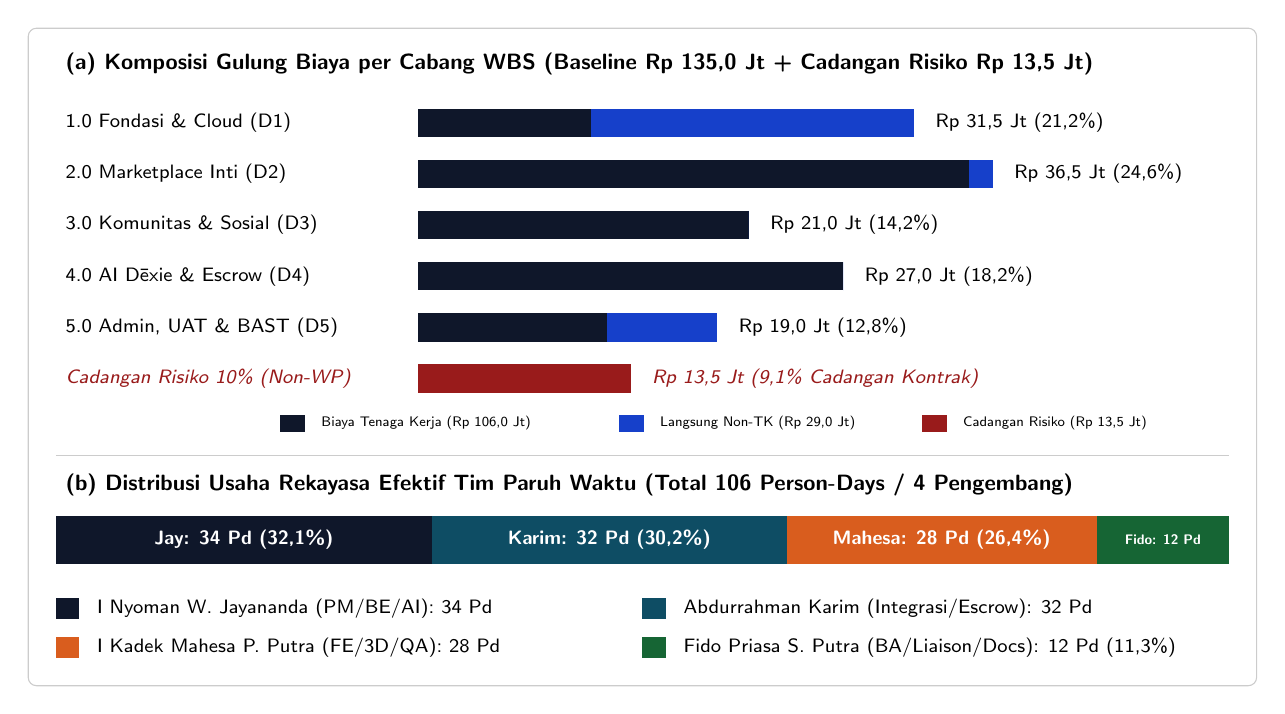
\begin{tikzpicture}[font=\sffamily]
    % Outer container card width 15.6cm
    \draw[bordergray, rounded corners=3pt] (0,0) rectangle (15.6, 8.35);

    % ---- PANEL A: Cost Baseline Roll-up by Branch + Contingency (top half y=4.05..8.15) ----
    \node[anchor=west, font=\sffamily\footnotesize\bfseries, text=black] at (0.35, 7.90) {(a) Komposisi Gulung Biaya per Cabang WBS (Baseline Rp 135,0 Jt + Cadangan Risiko Rp 13,5 Jt)};

    % Scale: max 40 Jt -> bar width 8.0cm (scale 0.20 cm/Jt at x=4.95 .. 12.95)
    \foreach \y/\lbl/\labval/\nonlabval/\totstr in {
        7.15/{1.0 Fondasi \& Cloud (D1)}/2.20/4.10/{Rp 31,5 Jt (21,2\%)},
        6.50/{2.0 Marketplace Inti (D2)}/7.00/0.30/{Rp 36,5 Jt (24,6\%)},
        5.85/{3.0 Komunitas \& Sosial (D3)}/4.20/0.00/{Rp 21,0 Jt (14,2\%)},
        5.20/{4.0 AI D\={e}xie \& Escrow (D4)}/5.40/0.00/{Rp 27,0 Jt (18,2\%)},
        4.55/{5.0 Admin, UAT \& BAST (D5)}/2.40/1.40/{Rp 19,0 Jt (12,8\%)}%
    } {
        \node[anchor=west, font=\sffamily\scriptsize, text=black] at (0.35, \y) {\lbl};
        \fill[brandnavy] (4.95, \y-0.18) rectangle ({4.95+\labval}, \y+0.18);
        \fill[brandblue] ({4.95+\labval}, \y-0.18) rectangle ({4.95+\labval+\nonlabval}, \y+0.18);
        \node[anchor=west, font=\sffamily\scriptsize, text=black] at ({5.10+\labval+\nonlabval}, \y) {\totstr};
    }
    % Contingency Reserve bar (13.5 * 0.20 = 2.70 cm)
    \node[anchor=west, font=\sffamily\scriptsize\itshape, text=accentred] at (0.35, 3.90) {Cadangan Risiko 10\% (Non-WP)};
    \fill[accentred] (4.95, 3.72) rectangle ({4.95+2.70}, 4.08);
    \node[anchor=west, font=\sffamily\scriptsize\itshape, text=accentred] at ({5.10+2.70}, 3.90) {Rp 13,5 Jt (9,1\% Cadangan Kontrak)};

    % Mini Legend Panel A (cleanly inset inside container x=3.20..15.25)
    \fill[brandnavy] (3.20, 3.22) rectangle (3.52, 3.44);
    \node[anchor=west, font=\sffamily\tiny, text=black] at (3.60, 3.33) {Biaya Tenaga Kerja (Rp 106,0 Jt)};
    \fill[brandblue] (7.50, 3.22) rectangle (7.82, 3.44);
    \node[anchor=west, font=\sffamily\tiny, text=black] at (7.90, 3.33) {Langsung Non-TK (Rp 29,0 Jt)};
    \fill[accentred] (11.35, 3.22) rectangle (11.67, 3.44);
    \node[anchor=west, font=\sffamily\tiny, text=black] at (11.75, 3.33) {Cadangan Risiko (Rp 13,5 Jt)};

    \draw[bordergray] (0.35, 2.92) -- (15.25, 2.92);

    % ---- PANEL B: 106 Pd Allocation across 4 Developers ----
    \node[anchor=west, font=\sffamily\footnotesize\bfseries, text=black] at (0.35, 2.55) {(b) Distribusi Usaha Rekayasa Efektif Tim Paruh Waktu (Total 106 \textit{Person-Days} / 4 Pengembang)};

    % Stacked bar spanning x=0.35 .. 15.25 (total width 14.90cm):
    % Jay 34/106=4.78, Karim 32/106=4.50, Mahesa 28/106=3.94, Fido 12/106=1.68 -> 4.78+4.50+3.94+1.68 = 14.90
    \fill[brandnavy] (0.35, 1.55) rectangle (5.13, 2.15);
    \fill[accentteal] (5.13, 1.55) rectangle (9.63, 2.15);
    \fill[accentorange] (9.63, 1.55) rectangle (13.57, 2.15);
    \fill[accentgreen] (13.57, 1.55) rectangle (15.25, 2.15);

    \node[white, font=\sffamily\scriptsize\bfseries] at (2.74, 1.85) {Jay: 34 Pd (32,1\%)};
    \node[white, font=\sffamily\scriptsize\bfseries] at (7.38, 1.85) {Karim: 32 Pd (30,2\%)};
    \node[white, font=\sffamily\scriptsize\bfseries] at (11.60, 1.85) {Mahesa: 28 Pd (26,4\%)};
    \node[white, font=\sffamily\tiny\bfseries] at (14.41, 1.85) {Fido: 12 Pd};

    % Bottom detail legend Panel B
    \fill[brandnavy] (0.35, 0.85) rectangle (0.65, 1.12);
    \node[anchor=west, font=\sffamily\scriptsize, text=black] at (0.75, 0.98) {I Nyoman W. Jayananda (PM/BE/AI): 34 Pd};
    \fill[accentteal] (7.80, 0.85) rectangle (8.10, 1.12);
    \node[anchor=west, font=\sffamily\scriptsize, text=black] at (8.20, 0.98) {Abdurrahman Karim (Integrasi/Escrow): 32 Pd};
    \fill[accentorange] (0.35, 0.35) rectangle (0.65, 0.62);
    \node[anchor=west, font=\sffamily\scriptsize, text=black] at (0.75, 0.48) {I Kadek Mahesa P. Putra (FE/3D/QA): 28 Pd};
    \fill[accentgreen] (7.80, 0.35) rectangle (8.10, 0.62);
    \node[anchor=west, font=\sffamily\scriptsize, text=black] at (8.20, 0.48) {Fido Priasa S. Putra (BA/Liaison/Docs): 12 Pd (11,3\%)};
\end{tikzpicture}
\caption{Visualisasi Gulung Biaya Baseline dan Distribusi Usaha Tim Rekayasa 106 \textit{Person-Days}}
\label{fig:cost_effort_rollup}
\end{figure}

\clearpage

% ==============================================================================
% BAB 4: ALUR KETERGANTUNGAN ANTAR-PAKET KERJA & JALUR KRITIS
% ==============================================================================
\section{Peta Ketergantungan Kerja dan Jalur Kritis}

Untuk mengoptimalkan paralelisme pengembangan pada tim paruh waktu, \figurename~\ref{fig:dependency_network} memetakan ketergantungan antarpaket kerja lintas lima fase rilis beserta penandaan Jalur Kritis (\textit{Critical Path}) dan batas lingkup cetak klien. Jalur kritis membentang pada rantai teknis: \textbf{1.1.1 $\rightarrow$ 1.3.1 $\rightarrow$ 1.4.1 $\rightarrow$ 2.1.2 $\rightarrow$ 2.3.2 $\rightarrow$ 4.2.2 $\rightarrow$ 4.3.2 $\rightarrow$ 5.2.2 $\rightarrow$ 5.3.2}.

\begin{figure}[H]
\centering
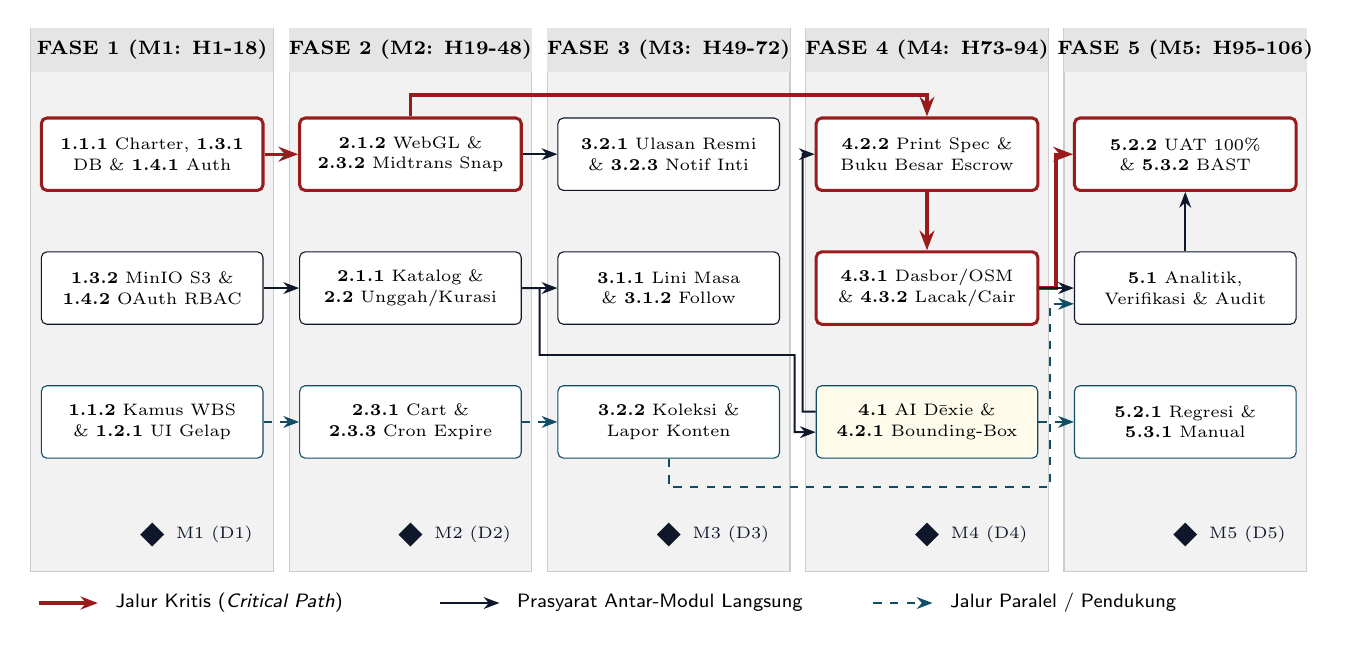
\begin{tikzpicture}[font=\sffamily, node distance=0.45cm]
    % Background phase swimlanes across 16.2cm (each col ~3.10cm + gap 0.17cm)
    \foreach \x/\title in {
        0.00/FASE 1 (M1: H1-18),
        3.28/FASE 2 (M2: H19-48),
        6.56/FASE 3 (M3: H49-72),
        9.84/FASE 4 (M4: H73-94),
        13.12/{FASE 5 (M5: H95-106)}%
    } {
        \fill[lightslate] (\x, 0.45) rectangle ({\x+3.08}, 7.35);
        \draw[bordergray] (\x, 0.45) rectangle ({\x+3.08}, 7.35);
        \fill[tableheadergray] (\x, 6.80) rectangle ({\x+3.08}, 7.35);
        \node[font=\fontsize{6.6}{7.5}\selectfont\bfseries, text=black] at ({\x+1.54}, 7.075) {\title};
    }

    % Define style macros inside scope via explicit nodes
    % Row y=5.75: Critical Path Spine (Accent Red border, white fill, bold code)
    % Row y=4.05: Primary Functional Track (Navy border)
    % Row y=2.35: Secondary Parallel Track (Teal/Muted border)
    % Row y=0.95: Milestone diamond markers

    % Col 1 (x_c = 1.54)
    \node[draw=accentred, line width=1.1pt, fill=white, rounded corners=2pt, text width=2.58cm, align=center, font=\fontsize{6.3}{7.4}\selectfont, minimum height=0.92cm] (n131) at (1.54, 5.75)
         {\textbf{1.1.1} Charter, \textbf{1.3.1} DB \& \textbf{1.4.1} Auth};
    \node[draw=brandnavy, fill=white, rounded corners=2pt, text width=2.58cm, align=center, font=\fontsize{6.3}{7.4}\selectfont, minimum height=0.92cm] (n132) at (1.54, 4.05)
         {\textbf{1.3.2} MinIO S3 \& \textbf{1.4.2} OAuth RBAC};
    \node[draw=accentteal, fill=white, rounded corners=2pt, text width=2.58cm, align=center, font=\fontsize{6.3}{7.4}\selectfont, minimum height=0.92cm] (n111) at (1.54, 2.35)
         {\textbf{1.1.2} Kamus WBS \& \textbf{1.2.1} UI Gelap};

    % Col 2 (x_c = 4.82)
    \node[draw=accentred, line width=1.1pt, fill=white, rounded corners=2pt, text width=2.58cm, align=center, font=\fontsize{6.3}{7.4}\selectfont, minimum height=0.92cm] (n232) at (4.82, 5.75)
         {\textbf{2.1.2} WebGL \& \textbf{2.3.2} Midtrans Snap};
    \node[draw=brandnavy, fill=white, rounded corners=2pt, text width=2.58cm, align=center, font=\fontsize{6.3}{7.4}\selectfont, minimum height=0.92cm] (n212) at (4.82, 4.05)
         {\textbf{2.1.1} Katalog \& \textbf{2.2} Unggah/Kurasi};
    \node[draw=accentteal, fill=white, rounded corners=2pt, text width=2.58cm, align=center, font=\fontsize{6.3}{7.4}\selectfont, minimum height=0.92cm] (n233) at (4.82, 2.35)
         {\textbf{2.3.1} Cart \& \textbf{2.3.3} Cron Expire};

    % Col 3 (x_c = 8.10)
    \node[draw=brandnavy, fill=white, rounded corners=2pt, text width=2.58cm, align=center, font=\fontsize{6.3}{7.4}\selectfont, minimum height=0.92cm] (n323) at (8.10, 5.75)
         {\textbf{3.2.1} Ulasan Resmi \& \textbf{3.2.3} Notif Inti};
    \node[draw=brandnavy, fill=white, rounded corners=2pt, text width=2.58cm, align=center, font=\fontsize{6.3}{7.4}\selectfont, minimum height=0.92cm] (n311) at (8.10, 4.05)
         {\textbf{3.1.1} Lini Masa \& \textbf{3.1.2} Follow};
    \node[draw=accentteal, fill=white, rounded corners=2pt, text width=2.58cm, align=center, font=\fontsize{6.3}{7.4}\selectfont, minimum height=0.92cm] (n322) at (8.10, 2.35)
         {\textbf{3.2.2} Koleksi \& Lapor Konten};

    % Col 4 (x_c = 11.38)
    \node[draw=accentred, line width=1.1pt, fill=white, rounded corners=2pt, text width=2.58cm, align=center, font=\fontsize{6.3}{7.4}\selectfont, minimum height=0.92cm] (n422) at (11.38, 5.75)
         {\textbf{4.2.2} Print Spec \& Buku Besar Escrow};
    \node[draw=accentred, line width=1.1pt, fill=white, rounded corners=2pt, text width=2.58cm, align=center, font=\fontsize{6.3}{7.4}\selectfont, minimum height=0.92cm] (n432) at (11.38, 4.05)
         {\textbf{4.3.1} Dasbor/OSM \& \textbf{4.3.2} Lacak/Cair};
    \node[draw=accentteal, fill=softamber, rounded corners=2pt, text width=2.58cm, align=center, font=\fontsize{6.3}{7.4}\selectfont, minimum height=0.92cm] (n41) at (11.38, 2.35)
         {\textbf{4.1} AI D\={e}xie \& \textbf{4.2.1} Bounding-Box};

    % Col 5 (x_c = 14.66)
    \node[draw=accentred, line width=1.1pt, fill=white, rounded corners=2pt, text width=2.58cm, align=center, font=\fontsize{6.3}{7.4}\selectfont, minimum height=0.92cm] (n522) at (14.66, 5.75)
         {\textbf{5.2.2} UAT 100\% \& \textbf{5.3.2} BAST};
    \node[draw=brandnavy, fill=white, rounded corners=2pt, text width=2.58cm, align=center, font=\fontsize{6.3}{7.4}\selectfont, minimum height=0.92cm] (n511) at (14.66, 4.05)
         {\textbf{5.1} Analitik, Verifikasi \& Audit};
    \node[draw=accentteal, fill=white, rounded corners=2pt, text width=2.58cm, align=center, font=\fontsize{6.3}{7.4}\selectfont, minimum height=0.92cm] (n531) at (14.66, 2.35)
         {\textbf{5.2.1} Regresi \& \textbf{5.3.1} Manual};

    % Critical Path solid thick crimson arrows (1.1.1 -> 1.3.1 -> 1.4.1 -> 2.1.2 -> 2.3.2 -> 4.2.2 -> 4.3.2 -> 5.2.2 -> 5.3.2)
    \draw[-{Stealth[length=2.5mm]}, accentred, line width=1.2pt] (n131.east) -- (n232.west);
    \draw[-{Stealth[length=2.5mm]}, accentred, line width=1.2pt] (n232.north) -- (4.82, 6.50) -- (11.38, 6.50) -- (n422.north);
    \draw[-{Stealth[length=2.5mm]}, accentred, line width=1.2pt] (n422.south) -- (n432.north);
    \draw[-{Stealth[length=2.5mm]}, accentred, line width=1.2pt] (n432.east) -- (13.02, 4.05) -- (13.02, 5.75) -- (n522.west);

    % Parallel & vertical dependency arrows (clean orthogonal corridor routing, zero crossings)
    \draw[-{Stealth[length=2mm]}, brandnavy, line width=0.7pt] (n232.east) -- (n323.west);
    \draw[-{Stealth[length=2mm]}, brandnavy, line width=0.7pt] (n132.east) -- (n212.west);
    \draw[-{Stealth[length=2mm]}, brandnavy, line width=0.7pt] (n212.east) -- (n311.west);
    \draw[-{Stealth[length=2mm]}, brandnavy, line width=0.7pt] (n212.east) -- (6.46, 4.05) -- (6.46, 3.20) -- (9.70, 3.20) -- (9.70, 2.22) -- ([yshift=-0.13cm]n41.west);
    \draw[-{Stealth[length=2mm]}, brandnavy, line width=0.7pt] ([yshift=0.13cm]n41.west) -- (9.80, 2.48) -- (9.80, 5.75) -- (n422.west);
    \draw[-{Stealth[length=2mm]}, brandnavy, line width=0.7pt] (n432.east) -- (n511.west);
    \draw[-{Stealth[length=2mm]}, brandnavy, line width=0.7pt] (n511.north) -- (n522.south);
    \draw[-{Stealth[length=2mm]}, accentteal, dashed, line width=0.7pt] (n111.east) -- (n233.west);
    \draw[-{Stealth[length=2mm]}, accentteal, dashed, line width=0.7pt] (n233.east) -- (n322.west);
    \draw[-{Stealth[length=2mm]}, accentteal, dashed, line width=0.7pt] (n322.south) -- (8.10, 1.52) -- (12.94, 1.52) -- (12.94, 3.85) -- ([yshift=-0.20cm]n511.west);
    \draw[-{Stealth[length=2mm]}, accentteal, dashed, line width=0.7pt] (n41.east) -- (n531.west);

    % Milestone gates at bottom y=0.92
    \foreach \xc/\mcode in {1.54/{M1 (D1)}, 4.82/{M2 (D2)}, 8.10/{M3 (D3)}, 11.38/{M4 (D4)}, 14.66/{M5 (D5)}} {
        \node[diamond, fill=brandnavy, inner sep=2.2pt] at (\xc, 0.92) {};
        \node[anchor=west, font=\fontsize{6.4}{7.5}\selectfont, text=brandnavy] at ({\xc+0.18}, 0.92) {\mcode};
    }

    % Legend under box
    \draw[-{Stealth[length=2.2mm]}, accentred, line width=1.2pt] (0.10, 0.05) -- (0.85, 0.05);
    \node[anchor=west, font=\sffamily\scriptsize, text=black] at (0.95, 0.05) {Jalur Kritis (\textit{Critical Path})};
    \draw[-{Stealth[length=2.0mm]}, brandnavy, line width=0.7pt] (5.20, 0.05) -- (5.95, 0.05);
    \node[anchor=west, font=\sffamily\scriptsize, text=black] at (6.05, 0.05) {Prasyarat Antar-Modul Langsung};
    \draw[-{Stealth[length=2.0mm]}, accentteal, dashed, line width=0.7pt] (10.70, 0.05) -- (11.45, 0.05);
    \node[anchor=west, font=\sffamily\scriptsize, text=black] at (11.55, 0.05) {Jalur Paralel / Pendukung};
\end{tikzpicture}
\caption{Diagram Jaringan Ketergantungan Antar-Paket Kerja \& Jalur Kritis Lintas Fase (M1 s.d. M5)}
\label{fig:dependency_network}
\end{figure}

\begin{table}[H]
\centering
\caption{Ringkasan Gerbang Ketergantungan Teknis Kunci}
{\renewcommand{\arraystretch}{1.12}\footnotesize
\begin{tabularx}{\textwidth}{| C{2.2cm} | C{2.2cm} | Y |}
\hline
\rowcolor{tableheadergray} \thdr{Paket Prasyarat} & \thdr{Paket Penerus} & \thdr{Rasional Ketergantungan Teknis} \\
\hline
1.3.1, 1.3.2 & 2.1.2, 2.2.1, 4.1.1 & Penyimpanan model 3D .glb dan indeks vektor pgvector tidak dapat diuji sebelum PostgreSQL dan klaster MinIO S3 aktif. \\
\hline
1.4.1, 1.4.2 & 2.2.1, 2.3.1, 3.1.1 & Pengendalian hak unggah kreator, checkout pembeli, dan sesi lini masa bergantung pada token JWT serta RBAC 5 peran. \\
\hline
2.3.2, 2.3.3 & 3.2.1, 4.2.2 & Ulasan pembeli resmi (\textit{verified purchase}) dan pencairan saldo cetak fisik memerlukan status pesanan lunas atomik (PAID). \\
\hline
4.2.1, 4.2.2 & 4.3.1, 4.3.2 & Dasbor bengkel mitra serta pelacakan 5 tahap baru bermakna setelah data estimasi ukuran klien dan buku besar \textit{escrow} dibuat. \\
\hline
1.0 s.d. 5.1 & 5.2.2, 5.3.2 & Uji UAT 100\% dan penandatanganan BAST menuntut seluruh fitur inti D1 s.d. D4 serta moderasi Admin lulus regresi penuh. \\
\hline
\end{tabularx}}
\end{table}

\clearpage

% ==============================================================================
% BAB 5: KAMUS WBS LENGKAP (COMPLETE WBS DICTIONARY)
% ==============================================================================
\section{Kamus WBS Lengkap (\textit{Complete WBS Dictionary})}

Setiap kartu kamus berikut merincikan spesifikasi teknis, batas ruang lingkup, luaran terukur, dan kriteria penerimaan biner (\textit{Definition of Done}) bagi seluruh 31 \textit{Work Package} dari kode 1.1.1 hingga 5.3.2.

\subsection{Cabang 1.0: Tata Kelola Proyek, Fondasi Infrastruktur \& Akses Akun (D1)}

\wbscard{1.1.1 Dokumen Project Charter v1.0 \& Daftar Pemangku Kepentingan}{CA 1.1 | Minggu 1 (Hari 1-5) | M1}
{Fido (BA: 1 Pd)}{1 Pd | TK: Rp 1.000.000 | Non-TK: Rp 0 | Total: Rp 1.000.000}
{Menyusun, menyelaraskan, dan mengesahkan Project Charter komersial tertutup v1.0 (SDN-3DEX-PC-001) bersama identifikasi pemangku kepentingan (\textit{Stakeholder Register} \& \textit{Power/Interest Grid}) sesuai standar PMBOK 6 Proses 4.1 dan 13.1.}
{Luaran: Dokumen Charter bilingual PDF/DOCX ditandatangani Sponsor, RM/PM, serta \textit{On-Site Customer}. Batas: Hanya mencakup parameter dasar proyek komersial 3D\={e}x.}
{Charter disetujui tanpa revisi mayor pada Minggu 1; seluruh peran tim, batas lingkup, matriks RACI tunggal-A, dan plafon Rp 148,5 Jt disahkan.}
{Prasyarat: MoU KREA3D-SDN/XII/2025 | Risiko Terkait: R-02 (\textit{Scope Creep}), R-06.}

\wbscard{1.1.2 Baseline Ruang Lingkup, Kamus WBS \& Model Domain UML}{CA 1.1 | Minggu 2-3 (Hari 6-18) | M1}
{Fido (BA: 2 Pd)}{2 Pd | TK: Rp 2.000.000 | Non-TK: Rp 0 | Total: Rp 2.000.000}
{Memecah kebutuhan pengguna menjadi struktur WBS 4 tingkat (SDN-3DEX-WBS-001), menyusun Kamus WBS untuk 31 WP, serta mendokumentasikan arsitektur monolith 4-node, ERD, Use Case, Activity, dan Sequence diagram.}
{Luaran: Dokumen Scope Baseline WBS lengkap, bagan hierarki, dan diagram UML tersinkronisasi (Print Spec, Job Queue). Batas: Tanpa \textit{G-code slicing} di server.}
{100\% cabang lingkup terlacak ke tujuan O-1 s.d. O-5; hasil gulung WP tepat 106 Pd dan Cost Baseline Rp 135 Jt tanpa selisih.}
{Prasyarat: 1.1.1 | Risiko Terkait: R-02, R-05.}

\wbscard{1.2.1 Prototipe Interaktif Antarmuka Tema Gelap \& Navigasi Responsif}{CA 1.2 | Minggu 2-3 (Hari 8-18) | M1}
{Mahesa (FE: 2 Pd)}{2 Pd | TK: Rp 2.000.000 | Non-TK: Rp 4.000.000 (UI Kit) | Total: Rp 6.000.000}
{Merancang sistem tema gelap terpadu (\textit{brand navy}, aksen jingga/biru), tata letak kerangka halaman Next.js App Router, sidebar responsif desktop/ponsel, dan komponen dasar antarmuka.}
{Luaran: Paket komponen UI Tailwind CSS dan sketsa layar awal tervalidasi oleh perwakilan pengguna. Batas: Tidak membangun aplikasi seluler asli Android/iOS.}
{Tampilan responsif terbaca jernih pada resolusi desktop (1280px+) dan seluler (375px+) serta memperoleh persetujuan demo dari Ibu Rina.}
{Prasyarat: 1.1.1 | Risiko Terkait: R-06.}

\wbscard{1.3.1 Server Produksi, PostgreSQL pgvector, SSL \& Kuota API 12 Bulan}{CA 1.3 | Minggu 1-2 (Hari 3-12) | M1}
{Jay (BE: 1 Pd)}{1 Pd | TK: Rp 1.000.000 | Non-TK: Rp 16.500.000 (Cloud/API) | Total: Rp 17.500.000}
{Menyiapkan lingkungan runtime Node.js/Express dan Next.js, mengonfigurasi basis data terpusat PostgreSQL 16 dengan ekstensi pgvector, skema ORM Prisma terpadu, sertifikat SSL domain, serta aktivasi kredensial API Midtrans/Google 12 bulan.}
{Luaran: Basis data PostgreSQL terhubung Prisma, tabel inti termigrasi, serta server uji dan domain siap pakai. Batas: Tidak bermigrasi dari data sistem lama klien.}
{Kueri pengujian basis data \& pgvector berhasil berjalan, endpoint pemeriksaan kesehatan /health mengembalikan status HTTP 200, serta HTTPS aktif.}
{Prasyarat: 1.1.1 (Kredensial Klien) | Risiko Terkait: R-01.}

\wbscard{1.3.2 Klaster Penyimpanan Objek MinIO S3 \& Pipeline Berkas Media 3D}{CA 1.3 | Minggu 2-3 (Hari 9-18) | M1}
{Jay (BE: 1 Pd), Karim (Int: 1 Pd)}{2 Pd | TK: Rp 2.000.000 | Non-TK: Rp 0 | Total: Rp 2.000.000}
{Menyiapkan layanan penyimpanan objek MinIO S3 terpisah untuk berkas biner .glb/.gltf, gambar pratinjau katalog, foto bukti cetak, serta kebijakan CORS dan URL prabubuhan bertanda tangan (\textit{presigned URL}).}
{Luaran: Bucket MinIO terstruktur dan modul layanan backend storage aktif. Batas: Pembatasan unggahan model 3D maksimal $< 50$ MB per berkas.}
{Unggah dan unduh berkas biner uji .glb berjalan stabil dengan validasi tipe MIME dan batas ukuran tanpa kebocoran akses publik pada berkas berbayar.}
{Prasyarat: 1.3.1 | Risiko Terkait: R-04.}

\wbscard{1.4.1 Registrasi, Login Kredensial, Verifikasi JWT \& Keamanan 2FA}{CA 1.4 | Minggu 2-3 (Hari 10-18) | M1}
{Jay (BE: 1 Pd), Karim (Int: 1 Pd)}{2 Pd | TK: Rp 2.000.000 | Non-TK: Rp 0 | Total: Rp 2.000.000}
{Membangun layanan registrasi pengguna email, enkripsi kata sandi bcrypt, penerbitan/verifikasi token sesi JWT terenkripsi, opsi keamanan dua langkah (2FA), serta halaman pengaturan profil akun.}
{Luaran: Modul API /auth \& /users beserta halaman login/register frontend fungsional. Batas: Sesi standar web peramban, bukan SSO perusahaan eksternal.}
{Uji registrasi, login, refresh token, dan verifikasi kode 2FA lulus seluruh skenario negatif (kata sandi salah/token kedaluwarsa) pada demo M1.}
{Prasyarat: 1.3.1 | Risiko Terkait: R-05.}

\wbscard{1.4.2 Integrasi Login Google OAuth \& Kontrol Akses 5 Peran RBAC}{CA 1.4 | Minggu 3 (Hari 13-18) | M1}
{Karim (Int: 1 Pd)}{1 Pd | TK: Rp 1.000.000 | Non-TK: Rp 0 | Total: Rp 1.000.000}
{Mengintegrasikan alur masuk satu klik via Google OAuth 2.0 dan menerapkan pembatasan rute antarmuka maupun middleware backend secara ketat untuk lima peran utama (\textit{Guest, Customer, Artist, Print Provider, Admin}).}
{Luaran: Middleware otorisasi RBAC aktif pada seluruh rute API serta tombol Login Google berfungsi penuh. Batas: Mengikuti kuota OAuth standar Google.}
{Setiap peran yang tidak berwenang mengakses rute terproteksi (mis. Customer mengakses rute /admin) ditolak otomatis dengan status HTTP 403.}
{Prasyarat: 1.4.1 | Risiko Terkait: R-01, R-05.}

\clearpage

\subsection{Cabang 2.0: Platform Inti Marketplace Aset 3D \& Integrasi Pembayaran (D2)}

\wbscard{2.1.1 Halaman Beranda, Katalog Kategori \& Mesin Filter Pencarian Publik}{CA 2.1 | Minggu 4-5 (Hari 19-30) | M2}
{Mahesa (FE: 3 Pd), Karim (Int: 2 Pd)}{5 Pd | TK: Rp 5.000.000 | Non-TK: Rp 0 | Total: Rp 5.000.000}
{Membangun halaman utama (\textit{landing page}) 3 pilar layanan (Model 3D, Tekstur, Jasa Cetak), daftar katalog publik dengan pagination ringan berbasis gambar pratinjau 2D, filter kategori/harga/lisensi, dan bilah pencarian cepat.}
{Luaran: Rute /catalog \& API pencarian terfilter terindeks rapi di PostgreSQL. Batas: Pencarian berbasis teks/atribut standar (pencarian vektor AI pada Cabang 4.1).}
{Halaman katalog terbuka $\le 3$ detik menggunakan peramban standar tanpa memuat mesh 3D berat secara massal pada daftar pratinjau (Tujuan O-1).}
{Prasyarat: 1.2.1, 1.3.2 | Risiko Terkait: R-04.}

\wbscard{2.1.2 Penampil 3D WebGL Interaktif (< 50 MB) \& Halaman Detail Aset}{CA 2.1 | Minggu 4-6 (Hari 20-38) | M2}
{Mahesa (FE: 5 Pd), Jay (BE: 2 Pd)}{7 Pd | TK: Rp 7.000.000 | Non-TK: Rp 1.500.000 (Uji 3D) | Total: Rp 8.500.000}
{Mengembangkan komponen kanvas WebGL interaktif menggunakan React Three Fiber / Three.js untuk memutar (\textit{orbit}), menggeser (\textit{pan}), dan memperbesar (\textit{zoom}) model .glb/.gltf langsung di browser beserta rincian metadata aset, tag, dan tombol aksi beli.}
{Luaran: Halaman detail model dengan penampil 3D mulus dan kendali pencahayaan dasar. Batas: Tanpa fitur \textit{Augmented Reality} khusus ponsel.}
{Penampil geometri 3D siap diinspeksi dalam waktu $\le 5$ detik untuk model berukuran $< 50$ MB pada desktop dan ponsel tanpa galat WebGL (Tujuan O-1).}
{Prasyarat: 1.3.2, 2.1.1 | Risiko Terkait: R-04.}

\wbscard{2.2.1 Portal Kreator: Unggah Aset .glb/.gltf \& Pengaturan Lisensi Ganda}{CA 2.2 | Minggu 5-6 (Hari 25-39) | M2}
{Jay (BE: 3 Pd), Mahesa (FE: 2 Pd)}{5 Pd | TK: Rp 5.000.000 | Non-TK: Rp 0 | Total: Rp 5.000.000}
{Menyediakan formulir unggah model 3D maupun paket tekstur bagi peran \textit{Artist}, ekstraksi metadata dimensi/format, unggah gambar pratinjau, serta opsi penetapan harga dan lisensi ganda (Gratis, Penggunaan Pribadi, dan Penggunaan Komersial).}
{Luaran: Rute backend /models \& antarmuka Studio Unggah Kreator. Batas: Hanya menerima format terstandar (.glb/.gltf, gambar pratinjau) di bawah batas ukuran.}
{Kreator berhasil mengunggah aset baru tersimpan ke MinIO S3 beserta entri metadata Prisma berstatus PENDING\_APPROVAL sebelum tayang ke publik.}
{Prasyarat: 1.3.2, 1.4.2 | Risiko Terkait: R-04, R-05.}

\wbscard{2.2.2 Antrean Kurasi Model Admin \& Tautan Unduhan Berbatas Waktu}{CA 2.2 | Minggu 5-7 (Hari 28-44) | M2}
{Jay (BE: 2 Pd), Karim (Int: 2 Pd), Fido (BA: 1 Pd)}{5 Pd | TK: Rp 5.000.000 | Non-TK: Rp 0 | Total: Rp 5.000.000}
{Membangun alur peninjauan aset baru oleh Admin (setujui/tolak dengan alasan) serta mekanisme perpustakaan pembeli (\textit{My Library}) yang menerbitkan tautan unduhan sementara (\textit{presigned URL}) khusus bagi pemegang hak beli sah.}
{Luaran: Antrean kurasi model dan layanan unduhan berhak akses (/purchases). Batas: Pembeli tidak dapat membagikan tautan permanen berkas mentah.}
{Pengguna tanpa bukti pembelian ditolak saat meminta unduhan; pembeli sah menerima berkas 3D melalui tautan kedaluwarsa terenkripsi.}
{Prasyarat: 2.2.1 | Risiko Terkait: R-05.}

\wbscard{2.3.1 Modul Keranjang Belanja, Daftar Keinginan (Wishlist) \& Ringkasan Order}{CA 2.3 | Minggu 5-6 (Hari 29-40) | M2}
{Karim (Int: 2 Pd), Mahesa (FE: 2 Pd)}{4 Pd | TK: Rp 4.000.000 | Non-TK: Rp 0 | Total: Rp 4.000.000}
{Mengembangkan layanan keranjang belanja persisten (/cart), manajemen daftar keinginan (/wishlist), validasi kepemilikan ganda agar pengguna tidak membeli lisensi identik dua kali, serta halaman ringkasan tagihan sebelum pembayaran.}
{Luaran: Antarmuka keranjang belanja, wishlist, dan kalkulasi subtotal/komisi bersih. Batas: Tanpa integrasi faktur pajak e-Faktur eksternal.}
{Item tertambah/terhapus secara sinkron antara Zustand dan PostgreSQL; kalkulasi total harga serta pilihan lisensi konsisten hingga tahap checkout.}
{Prasyarat: 1.4.1, 2.1.1 | Risiko Terkait: R-05.}

\wbscard{2.3.2 Pembayaran Midtrans Snap, Webhook Idempoten \& Transaksi Atomik}{CA 2.3 | Minggu 6-7 (Hari 34-46) | M2}
{Karim (Int: 3 Pd), Jay (BE: 2 Pd), Fido (BA: 1 Pd)}{6 Pd | TK: Rp 6.000.000 | Non-TK: Rp 0 | Total: Rp 6.000.000}
{Mengintegrasikan gerbang pembayaran Midtrans Snap, memverifikasi tanda tangan kriptografis webhook notifikasi pembayaran, dan mengeksekusi pembaruan tabel Order, Payment, serta Purchase dalam satu transaksi Prisma \$transaction atomik.}
{Luaran: Rute /orders dan /payments/webhook dengan mesin status pesanan (PENDING $\rightarrow$ PAID). Batas: Tanpa rekonsiliasi sistem akuntansi ERP eksternal.}
{Pencatatan transaksi berhasil $\ge 99{,}5\%$ tanpa tagihan atau hak beli ganda walau webhook dikirim ulang berkali-kali (uji \textit{idempotency} lulus, Tujuan O-3).}
{Prasyarat: 1.3.1, 2.3.1 | Risiko Terkait: R-01, R-05.}

\wbscard{2.3.3 Penjadwal Otomatis Pembatalan Checkout Kedaluwarsa \& Token Sesi}{CA 2.3 | Minggu 7 (Hari 41-48) | M2}
{Jay (BE: 2 Pd), Karim (Int: 1 Pd)}{3 Pd | TK: Rp 3.000.000 | Non-TK: Rp 0 | Total: Rp 3.000.000}
{Mengimplementasikan layanan penjadwal waktu berkala internal (\textit{cron scheduler}) sebagai aktor sistem untuk membatalkan otomatis pesanan Midtrans berstatus PENDING yang melewati tenggat kedaluwarsa (CANCELLED) serta membersihkan token sesi usang.}
{Luaran: Tugas latar belakang penjadwal transaksi kedaluwarsa aktif di modul backend. Batas: Penjadwal berjalan di proses backend monolith tanpa antrean terpisah eksternal.}
{Pesanan uji yang dibiarkan melampaui batas waktu pembayaran Midtrans otomatis berubah status menjadi CANCELLED dan riwayat keranjang tetap bersih pada demo M2.}
{Prasyarat: 2.3.2 | Risiko Terkait: R-05.}

\clearpage

\subsection{Cabang 3.0: Ekosistem Komunitas, Interaksi Sosial \& Notifikasi (D3)}

\wbscard{3.1.1 Lini Masa Publikasi Portofolio Kreator, Suka \& Thread Komentar}{CA 3.1 | Minggu 8-9 (Hari 49-59) | M3}
{Jay (BE: 2 Pd), Karim (Int: 2 Pd), Mahesa (FE: 1 Pd)}{5 Pd | TK: Rp 5.000.000 | Non-TK: Rp 0 | Total: Rp 5.000.000}
{Membangun ruang komunitas terpadu (/posts) tempat kreator memublikasikan pembaruan karya 3D beserta gambar render/tautan katalog, mendukung interaksi suka (\textit{like}) dan utas komentar bertingkat antaranggota.}
{Luaran: Halaman lini masa komunitas dan modul API posting, like, serta komentar. Batas: Tanpa fitur pesan obrolan video/suara langsung (\textit{real-time call}).}
{Pengguna terautentikasi dapat membuat unggahan portofolio, menyukai, menyunting, dan mengomentari postingan secara persisten tanpa galat tata letak.}
{Prasyarat: 1.4.2, 2.2.1 | Risiko Terkait: R-05.}

\wbscard{3.1.2 Modul Profil Publik Kreator \& Mekanisme Ikuti (Follow/Unfollow)}{CA 3.1 | Minggu 8-9 (Hari 52-62) | M3}
{Karim (Int: 2 Pd), Mahesa (FE: 1 Pd)}{3 Pd | TK: Rp 3.000.000 | Non-TK: Rp 0 | Total: Rp 3.000.000}
{Mengembangkan halaman profil publik kreator dan mitra cetak yang menampilkan portofolio karya, statistik pengikut, serta fitur ikuti/berhenti mengikuti (/follow) untuk mempersonalisasi lini masa.}
{Luaran: Rute profil publik dan API grafik relasi pengikut. Batas: Tidak mengimpor grafik pengikut dari media sosial eksternal.}
{Aksi \textit{follow/unfollow} memperbarui jumlah pengikut secara atomik dan menyaring feed komunitas sesuai daftar kreator yang diikuti.}
{Prasyarat: 1.4.1, 3.1.1 | Risiko Terkait: R-05.}

\wbscard{3.2.1 Sistem Ulasan \& Penilaian Aset Pembeli Resmi (Verified Purchase)}{CA 3.2 | Minggu 9-10 (Hari 60-68) | M3}
{Karim (Int: 2 Pd), Jay (BE: 1 Pd), Fido (BA: 1 Pd)}{4 Pd | TK: Rp 4.000.000 | Non-TK: Rp 0 | Total: Rp 4.000.000}
{Membangun modul ulasan bintang dan komentar kualitas aset (/reviews) yang hanya mengizinkan pengguna dengan catatan kepemilikan pembelian terkonfirmasi (PAID) untuk mencegah ulasan palsu, lengkap dengan penghitungan rata-rata skor aset.}
{Luaran: Form \& daftar ulasan terverifikasi pada halaman detail aset serta API validasi kepemilikan. Batas: Satu ulasan sah per aset terbeli.}
{Pengguna yang belum membeli model ditolak oleh server (HTTP 403); pembeli resmi dapat mengirim ulasan yang langsung memperbarui peringkat rata-rata model.}
{Prasyarat: 2.3.2 | Risiko Terkait: R-05.}

\wbscard{3.2.2 Pengelolaan Koleksi Kurasi Pribadi/Publik \& Pelaporan Konten}{CA 3.2 | Minggu 9-10 (Hari 60-70) | M3}
{Jay (BE: 2 Pd), Mahesa (FE: 1 Pd), Fido (BA: 1 Pd)}{4 Pd | TK: Rp 4.000.000 | Non-TK: Rp 0 | Total: Rp 4.000.000}
{Menyediakan fitur koleksi papan inspirasi kurasi (/collections) bagi pembeli untuk mengelompokkan aset favorit (pribadi/publik) serta formulir pelaporan pelanggaran hak cipta atau konten tidak pantas (/reports) dari komunitas/katalog.}
{Luaran: Antarmuka pengelola koleksi pengguna dan saluran pembuatan tiket laporan pelanggaran. Batas: Resolusi sengketa DMCA kompleks ditangani manual Admin.}
{Pengguna dapat menambah/menghapus model dari koleksi serta mengirim laporan pelanggaran yang langsung masuk ke antrean Admin.}
{Prasyarat: 2.1.1, 3.1.1 | Risiko Terkait: R-05.}

\wbscard{3.2.3 Layanan Pusat Notifikasi In-App \& Log Aktivitas Transaksional}{CA 3.2 | Minggu 9-10 (Hari 63-72) | M3}
{Karim (Int: 3 Pd), Jay (BE: 2 Pd)}{5 Pd | TK: Rp 5.000.000 | Non-TK: Rp 0 | Total: Rp 5.000.000}
{Mengembangkan modul pusat notifikasi internal (/notification) untuk memberi tahu peristiwa penjualan model, persetujuan kurasi Admin, komentar baru, pengikut baru, dan perubahan status pesanan cetak dengan status baca/belum baca.}
{Luaran: Lonceng notifikasi interaktif di header, panel riwayat notifikasi, dan pemicu notifikasi otomatis lintas modul. Batas: Tanpa pengiriman SMS berbayar atau notifikasi \textit{push} aplikasi asli.}
{Setiap peristiwa transaksi maupun sosial memicu entri notifikasi yang tepat sasaran dan dapat ditandai telah dibaca pada demonstrasi M3.}
{Prasyarat: 2.3.2, 3.1.1, 3.2.1 | Risiko Terkait: R-05.}

\vspace{4pt}

\subsection{Cabang 4.0: Asisten Cerdas AI D\={e}xie \& Layanan Cetak 3D Escrow (D4)}

\wbscard{4.1.1 Pipeline Embedding Vektor Lokal \& Kueri Kosinus pgvector}{CA 4.1 | Minggu 11-12 (Hari 73-84) | M4}
{Jay (BE: 4 Pd), Mahesa (FE: 1 Pd)}{5 Pd | TK: Rp 5.000.000 | Non-TK: Rp 0 | Total: Rp 5.000.000}
{Mengimplementasikan pembangkitan vektor embedding metadata model 3D menggunakan pustaka Transformers.js lokal secara asinkron saat aset disetujui, menyimpan vektor berdimensi tetap di kolom pgvector, dan membangun kueri kesamaan jarak kosinus untuk pencarian semantik.}
{Luaran: Indeks pencarian vektor pgvector aktif dan layanan pencari kemiripan kontekstual. Batas: Tidak melakukan pemindaian citra mesh mentah 3D secara langsung untuk embedding.}
{Kueri pencarian semantik mengembalikan kandidat model relevan beserta skor kedekatan vektor dalam waktu respons server $< 0{,}5$ detik (Tujuan O-4).}
{Prasyarat: 1.3.1, 2.2.2 | Risiko Terkait: R-04, R-05.}

\wbscard{4.1.2 Penalaran Kontekstual Gemini API \& Panel Asisten Interaktif D\={e}xie}{CA 4.1 | Minggu 11-12 (Hari 76-88) | M4}
{Jay (BE: 2 Pd), Mahesa (FE: 2 Pd)}{4 Pd | TK: Rp 4.000.000 | Non-TK: Rp 0 | Total: Rp 4.000.000}
{Mengintegrasikan layanan Google Gemini API (/dexie) untuk menghasilkan saran konteks model 3D, menjawab pertanyaan kesesuaian cetak aset secara alami, serta menampilkan panel asisten AI D\={e}xie yang dapat dinyalakan/dimatikan sesuai preferensi pengguna.}
{Luaran: Widget asisten D\={e}xie di halaman detail model dan pencari rekomendasi cerdas dengan fallback aman saat kuota AI terbatas. Batas: Mengandalkan ketersediaan API Google Gemini.}
{Panel D\={e}xie merespons pertanyaan konteks model $\le 0{,}5$ detik untuk retrieval konteks katalog dan menampilkan pesan cadangan anggun bila layanan AI eksternal mengalami gangguan (R-01).}
{Prasyarat: 4.1.1 | Risiko Terkait: R-01, R-05.}

\wbscard{4.2.1 Form Konfigurasi Cetak 3D \& Estimasi Dimensi/Volume Sisi Klien}{CA 4.2 | Minggu 11-12 (Hari 75-87) | M4}
{Mahesa (FE: 3 Pd), Karim (Int: 1 Pd), Fido (BA: 1 Pd)}{5 Pd | TK: Rp 5.000.000 | Non-TK: Rp 0 | Total: Rp 5.000.000}
{Membangun halaman pemesanan cetak fisik (/print) meliputi kalkulasi dimensi dan perkiraan volume berbasis kotak pembatas (\textit{bounding-box estimation}) langsung di browser pengguna, disertai pilihan skala, jenis bahan (PLA, ABS, Resin SLA, TPU, Nylon SLS), kepadatan \textit{infill}, dan warna.}
{Luaran: Kalkulator estimasi biaya cetak sisi klien real-time tanpa proses potong jalur cetak di server. Batas: Tidak mengoperasikan \textit{server-side G-code slicing engine} maupun kendali mesin IoT.}
{Perubahan skala, material, atau kepadatan memperbarui estimasi dimensi (mm) dan perkiraan harga cetak seketika di browser dengan akurat.}
{Prasyarat: 2.1.2 | Risiko Terkait: R-02, R-05.}

\wbscard{4.2.2 Layanan Print Spec, Job Queue \& Buku Besar Penahanan Saldo Escrow}{CA 4.2 | Minggu 12-13 (Hari 80-92) | M4}
{Jay (BE: 3 Pd), Karim (Int: 2 Pd)}{5 Pd | TK: Rp 5.000.000 | Non-TK: Rp 0 | Total: Rp 5.000.000}
{Membangun modul backend penyimpanan spesifikasi cetak (\textit{Print Spec}), manajemen antrean kerja mitra (\textit{Job Queue} pada /print), dan mekanisme buku besar penahanan saldo sementara (\textit{simple ledger/escrow}) berbasis status transaksi hingga konfirmasi pengiriman DELIVERED.}
{Luaran: Layanan API pesanan cetak terintegrasi transaksi Midtrans dan mekanisme pembekuan saldo mitra sampai barang diterima. Batas: Pencatatan ledger internal platform tanpa modul rekening giro perbankan terpisah.}
{Penerusan order lengkap (berkas + detail spesifikasi cetak) dari pembeli ke antrean mitra berjalan $\le 5$ menit (Tujuan O-2); saldo tertahan otomatis dan dapat direfund bila mitra menolak (R-07).}
{Prasyarat: 2.3.2, 4.2.1 | Risiko Terkait: R-05, R-07.}

\wbscard{4.3.1 Dasbor Mitra Cetak, Peta Geospasial Leaflet/OSM \& Unduh Kerja}{CA 4.3 | Minggu 12-13 (Hari 82-92) | M4}
{Karim (Int: 2 Pd), Mahesa (FE: 2 Pd)}{4 Pd | TK: Rp 4.000.000 | Non-TK: Rp 0 | Total: Rp 4.000.000}
{Mengembangkan dasbor antrean pesanan cetak khusus \textit{Print Provider} untuk menerima atau menolak pekerjaan masuk, mengunduh berkas .glb resmi pesanan secara aman, serta mengintegrasikan pemilih lokasi peta OpenStreetMap/Leaflet gratis guna menampilkan lokasi bengkel terdekat bagi pembeli.}
{Luaran: Antarmuka antrean pekerjaan Print Provider dan komponen peta Leaflet/OSM (LeafletMapInner). Batas: Tanpa pengadaan armada fisik atau mesin cetak milik platform.}
{Mitra cetak dapat melihat profil geografis bengkel di peta, mengklaim order cetak masuk, serta mengunduh model 3D terkait dalam antrean kerja tanpa error.}
{Prasyarat: 1.4.2, 4.2.2 | Risiko Terkait: R-05, R-07.}

\wbscard{4.3.2 Alur Status 5 Tahap, Bukti Foto Cetak, Resi \& Konfirmasi Escrow}{CA 4.3 | Minggu 13 (Hari 85-94) | M4}
{Karim (Int: 3 Pd), Fido (BA: 1 Pd)}{4 Pd | TK: Rp 4.000.000 | Non-TK: Rp 0 | Total: Rp 4.000.000}
{Mengimplementasikan pembaruan 5 tahap status order cetak (PENDING $\rightarrow$ PAID $\rightarrow$ PROCESSING $\rightarrow$ SHIPPED/DELIVERED $\rightarrow$ COMPLETED), unggah foto bukti fisik hasil cetakan oleh mitra, input manual nomor resi pengiriman, dan tombol konfirmasi penerimaan oleh Customer untuk melepas dana \textit{escrow}.}
{Luaran: Lini pelacakan status 5 tahap bagi Customer dan form unggah bukti + resi bagi Mitra Cetak. Batas: Tanpa integrasi API pelacakan kurir otomatis berbayar pihak ketiga.}
{Dana \textit{escrow} hanya berpindah ke saldo siap tarik mitra setelah status mencapai DELIVERED dan dikonfirmasi Customer (atau setelah batas otomatis 14 hari pada skenario M4).}
{Prasyarat: 4.3.1 | Risiko Terkait: R-06, R-07.}

\vspace{4pt}

\subsection{Cabang 5.0: Tata Kelola Admin, Penjaminan Mutu UAT \& Serah Terima Produksi (D5)}

\wbscard{5.1.1 Dasbor Analitik Pendapatan, Verifikasi Kreator \& Mitra Cetak}{CA 5.1 | Minggu 14 (Hari 95-100) | M5}
{Jay (BE: 2 Pd), Karim (Int: 1 Pd)}{3 Pd | TK: Rp 3.000.000 | Non-TK: Rp 0 | Total: Rp 3.000.000}
{Membangun dasbor statistik penjualan dan pendapatan kotor/komisi bagi Kreator maupun Admin (/analytics), dilengkapi antrean verifikasi persetujuan pengajuan peran baru Kreator 3D dan Mitra Jasa Cetak sebelum dapat bertransaksi komersial.}
{Luaran: Halaman statistik analitik transaksi dan panel verifikasi peran mitra di dasbor Admin. Batas: Laporan keuangan internal platform, bukan modul pajak akuntansi eksternal.}
{Seluruh metrik penjualan digital maupun jasa cetak dapat dipantau realtime 24 jam dengan kesesuaian angka transaksi 100\% terhadap database (Tujuan O-5).}
{Prasyarat: 2.3.2, 4.3.2 | Risiko Terkait: R-05.}

\wbscard{5.1.2 Moderasi Laporan Pelanggaran \& Catatan Audit Admin Permanen}{CA 5.1 | Minggu 14 (Hari 96-101) | M5}
{Jay (BE: 1 Pd), Karim (Int: 1 Pd)}{2 Pd | TK: Rp 2.000.000 | Non-TK: Rp 0 | Total: Rp 2.000.000}
{Membangun antrean penyelesaian laporan pelanggaran (/admin \& /reports), kewenangan penonaktifan akun/model pelanggar aturan, serta tabel log audit (Admin\_Audit\_Log) bersifat \textit{append-only} untuk mencatat setiap tindakan moderasi kritis.}
{Luaran: Antarmuka moderasi konten/akun Admin dan penampil catatan audit permanen. Batas: Catatan audit tidak dapat disunting atau dihapus oleh Admin biasa.}
{Setiap eksekusi ban pengguna, penghapusan aset, atau verifikasi mitra otomatis memicu pencatatan catatan audit lengkap (aktor, waktu, target, alasan) tanpa celah (Tujuan O-5).}
{Prasyarat: 3.2.2, 5.1.1 | Risiko Terkait: R-05.}

\wbscard{5.2.1 Eksekusi Pengujian Integrasi, Regresi Otomatis \& Uji Kecepatan Muat}{CA 5.2 | Minggu 14 (Hari 95-102) | M5}
{Mahesa (QA: 2 Pd)}{2 Pd | TK: Rp 2.000.000 | Non-TK: Rp 2.000.000 (QA Regresi) | Total: Rp 4.000.000}
{Menjalankan rangkaian uji otomatis endpoint backend, uji integrasi alur transaksi Midtrans/\textit{escrow}, uji silang kompatibilitas antarmuka pasca penguncian fitur (\textit{feature freeze} Hari ke-95), dan pengukuran kecepatan muat katalog \& penampil 3D.}
{Luaran: Laporan hasil uji regresi otomatis \& audit metrik performa (Tujuan O-1 s.d. O-5). Batas: Pengujian berfokus pada lingkup sistem produksi web 3D\={e}x.}
{Nol cacat kritis/tinggi tersisa pada fitur produksi; waktu muat katalog $\le 3$ dtk, penampil 3D $\le 5$ dtk, dan pencarian vektor $< 0{,}5$ dtk.}
{Prasyarat: Seluruh modul 1.0 s.d. 5.1 selesai \& \textit{Feature Freeze} Hari 95 | Risiko Terkait: R-02, R-04, R-05.}

\wbscard{5.2.2 Lokakarya Uji Penerimaan Pengguna (UAT) 100\% Lulus Tanpa Cacat}{CA 5.2 | Minggu 15 (Hari 100-104) | M5}
{Mahesa (QA: 1 Pd), Fido (BA: 1 Pd)}{2 Pd | TK: Rp 2.000.000 | Non-TK: Rp 0 | Total: Rp 2.000.000}
{Memfasilitasi uji penerimaan pengguna (\textit{User Acceptance Testing} / UAT) terstruktur bersama perwakilan pengguna dari Krea3D Corp (Ibu Rina serta penguji peran Pembeli, Kreator, Mitra Cetak, dan Admin) mencakup seluruh alur bisnis dari registrasi hingga pencairan \textit{escrow}.}
{Luaran: Lembar Berita Acara Skenario Uji UAT bertanda tangan perwakilan Krea3D Corp. Batas: Tidak menerima permintaan fitur baru di luar lingkup Charter v1.0.}
{100\% skenario uji UAT dinyatakan LULUS tanpa cacat kritis yang menghambat operasional peluncuran (Kriteria Sukses Charter).}
{Prasyarat: 5.2.1 | Risiko Terkait: R-02, R-06.}

\wbscard{5.3.1 Penyusunan Manual Pengguna/Admin \& Penyerahan Kode Tertutup}{CA 5.3 | Minggu 14-15 (Hari 98-104) | M5}
{Fido (BA: 1 Pd)}{1 Pd | TK: Rp 1.000.000 | Non-TK: Rp 2.500.000 (Dokumentasi) | Total: Rp 3.500.000}
{Menyusun buku panduan pengoperasian lengkap per peran pengguna (Pembeli, Kreator, Mitra Cetak, dan Administrator), panduan pemeliharaan server/basis data, serta menyiapkan bundel repositori kode sumber tertutup beserta dokumentasi API bagi Krea3D Corp.}
{Luaran: Manual Operasional PDF terstruktur dan paket arsip repositori kode tertutup eksklusif milik klien. Batas: Kode sumber dilarang dipublikasikan secara terbuka.}
{Manual diverifikasi dapat diikuti secara mandiri oleh staf non-teknis klien dan paket repositori lengkap diserahkan ke infrastruktur klien.}
{Prasyarat: 5.1.2, 5.2.1 | Risiko Terkait: R-05.}

\wbscard{5.3.2 Pelatihan Staf Krea3D, Peluncuran Produksi \& Pengesahan BAST}{CA 5.3 | Minggu 15 (Hari 103-106) | M5}
{Fido (BA: 1 Pd), Jay (PM: 1 Pd)}{2 Pd | TK: Rp 2.000.000 | Non-TK: Rp 2.500.000 (Pelatihan \& Serah Terima) | Total: Rp 4.500.000}
{Menyelenggarakan sesi pelatihan operasional langsung bagi tim operasional dan moderator Krea3D Corp, mengaktifkan platform secara penuh pada domain produksi https://3dex.studio, dan menandatangani Berita Acara Serah Terima (BAST) akhir proyek paling lambat Hari ke-106.}
{Luaran: Platform aktif di lingkungan produksi klien, daftar hadir pelatihan staf, dan BAST resmi ditandatangani Sponsor \& PM. Batas: Penutupan proyek formal per 20 April 2026.}
{Sistem berjalan stabil di produksi dengan ketersediaan $\ge 99{,}5\%$, total realisasi biaya tidak melampaui Rp 148.500.000, dan BAST disahkan tepat waktu.}
{Prasyarat: 5.2.2, 5.3.1 | Risiko Terkait: R-06.}

\vspace{8pt}

% ==============================================================================
% BAB 6: MATRIKS KETERLACAKAN, TATA KELOLA PERUBAHAN & REFERENSI STANDAR
% ==============================================================================
\section{Matriks Keterlacakan Lingkup dan Tata Kelola Perubahan}

\subsection{Matriks Keterlacakan (\textit{Requirements Traceability}: Charter SMART $\rightarrow$ WBS $\rightarrow$ RACI)}
Tabel \ref{tab:traceability} membuktikan setiap sasaran bisnis terukur (O-1 s.d. O-5) dan lima hasil serahan utama Charter (D1 s.d. D5) terlacak tuntas pada kelompok \textit{Work Package} spesifik beserta akuntabilitas tunggal (A) dan pelaksana utama (R) dari matriks RACI.

\begin{table}[H]
\centering
\caption{Matriks Keterlacakan Sasaran Charter, Serahan Utama, Kode WBS, dan Tanggung Jawab}
{\renewcommand{\arraystretch}{1.14}\footnotesize
\begin{tabularx}{\textwidth}{| C{1.3cm} | L{3.3cm} | C{1.3cm} | L{3.5cm} | C{1.8cm} | Y |}
\hline
\rowcolor{tableheadergray} \thdr{Tujuan Charter} & \thdr{Area \& Target Terukur} & \thdr{Serahan \& Tonggak} & \thdr{Komponen WBS Terkait} & \thdr{Pemegang A / R Utama} & \thdr{Metode Verifikasi Kelulusan} \\
\hline
O-1 & Kecepatan Katalog ($\le 3$ dtk) \& Penampil 3D ($\le 5$ dtk) & D1, D2 (M1, M2) & 1.2.1, 1.3.2, 2.1.1, 2.1.2, 5.2.1 & \textbf{A:} Mahesa \newline R: Karim, Jay & Pengukuran waktu muat Lighthouse/browser pada model $< 50$ MB sebelum rilis akhir. \\
\hline
O-2 & Alur Cetak Fisik ($\le 5$ mnt) \& Estimasi Sisi Klien & D4 (M4) & 4.2.1, 4.2.2, 4.3.1, 4.3.2 & \textbf{A:} Jay \newline R: Karim, Mahesa & Uji alur pengajuan spesifikasi cetak (\textit{bounding-box}) sampai muncul di antrean dasbor mitra. \\
\hline
O-3 & Keandalan Bayar ($\ge 99{,}5\%$, Nol Tagihan Ganda) & D2 (M2) & 2.3.1, 2.3.2, 2.3.3, 5.2.1 & \textbf{A:} Jay \newline R: Karim, Fido & Pengujian webhook Midtrans Snap berulang, transaksi atomik DB, dan uji kedaluwarsa cron. \\
\hline
O-4 & Pencarian AI D\={e}xie ($\le 0{,}5$ dtk) \& Konversi Naik $\ge 25\%$ & D4 (M4) & 1.3.1, 4.1.1, 4.1.2 & \textbf{A:} Jay \newline R: Mahesa & Uji latensi kueri kosinus pgvector dan demonstrasi interaksi asisten D\={e}xie. \\
\hline
O-5 & Dasbor Analitik, Moderasi \& Audit Permanen 24 Jam & D3, D5 (M3, M5) & 3.1.1 s.d. 3.2.3, 5.1.1, 5.1.2, 5.2.2, 5.3.2 & \textbf{A:} Jay \newline R: Karim, Mahesa, Fido & Audit integritas Admin\_Audit\_Log, uji UAT 100\% oleh klien, pelatihan, dan BAST. \\
\hline
\end{tabularx}}
\label{tab:traceability}
\end{table}

\clearpage

\subsection{Tata Kelola Pengendalian Perubahan Lingkup (\textit{Integrated Change Control})}
Setelah dokumen SDN-3DEX-WBS-001 disahkan sebagai \textit{Scope Baseline}, seluruh kode WBS 1.1.1 s.d. 5.3.2 bersifat mengikat. Setiap permintaan modifikasi atau penambahan fitur di luar daftar 31 \textit{Work Package} wajib mematuhi alur tata kelola berikut:
\begin{enumerate}[leftmargin=1.5em, itemsep=1.5pt]
    \item \textbf{Pengajuan \textit{Change Request}:} Diajukan tertulis oleh \textit{On-Site Customer} atau Sponsor sebelum batas penguncian fitur (\textit{feature freeze} Hari ke-95).
    \item \textbf{Analisis Dampak:} Project Manager (Jay) dan Business Analyst (Fido) menilai dampak perubahan terhadap lingkup, jadwal, kebutuhan \textit{person-days}, serta estimasi pencairan biaya addendum.
    \item \textbf{Persetujuan Berjenjang:} Perubahan baru sah dikerjakan apabila mendapat persetujuan tertulis bersama dari \textit{Executive Project Sponsor} (Ir. Hendra Wijaya) dan \textit{Project Manager}, diikuti pembaruan nomor versi pada Kamus WBS agar kepatuhan Aturan 100\% tetap terjaga.
\end{enumerate}

\subsection{Referensi Standar dan Dokumen Rujukan}
\begin{itemize}[leftmargin=1.5em, itemsep=1.5pt]
    \item Project Management Institute (PMI). (2017). \textit{A Guide to the Project Management Body of Knowledge (PMBOK\textsuperscript{\textregistered} Guide)}, 6th Edition. Bab 5 (\textit{Project Scope Management}, Proses 5.4 \textit{Create WBS}) dan Bab 7 (\textit{Project Cost Management}).
    \item Project Management Institute (PMI). (2019). \textit{Practice Standard for Work Breakdown Structures}, 3rd Edition. Panduan Aturan 100\%, \textit{Control Accounts}, \textit{Work Packages}, dan \textit{WBS Dictionary}.
    \item PT Schryzon Digital Nusantara. (2026). \textit{Project Charter v1.0: Platform Marketplace Aset 3D \& Ekosistem Cetak Fisik ``3D\={e}x''} (Dokumen Resmi Nomor SDN-3DEX-PC-001).
    \item Repositori Teknis Internal Platform 3D\={e}x (\textit{Modular Monolith Specification}, \textit{Prisma Database Schema}, dan Rute Layanan API Backend \& Frontend).
\end{itemize}

\end{document}
